\documentclass[]{book}
\usepackage{lmodern}
\usepackage{setspace}
\setstretch{2}
\usepackage{amssymb,amsmath}
\usepackage{ifxetex,ifluatex}
\usepackage{fixltx2e} % provides \textsubscript
\ifnum 0\ifxetex 1\fi\ifluatex 1\fi=0 % if pdftex
  \usepackage[T1]{fontenc}
  \usepackage[utf8]{inputenc}
\else % if luatex or xelatex
  \ifxetex
    \usepackage{mathspec}
  \else
    \usepackage{fontspec}
  \fi
  \defaultfontfeatures{Ligatures=TeX,Scale=MatchLowercase}
    \setmainfont[]{FreeSerif}
\fi
% use upquote if available, for straight quotes in verbatim environments
\IfFileExists{upquote.sty}{\usepackage{upquote}}{}
% use microtype if available
\IfFileExists{microtype.sty}{%
\usepackage{microtype}
\UseMicrotypeSet[protrusion]{basicmath} % disable protrusion for tt fonts
}{}
\usepackage[margin=1in]{geometry}
\usepackage{hyperref}
\hypersetup{unicode=true,
            pdftitle={Knowledge of the U.S. Social Sciences},
            pdfauthor={Brooks Ambrose},
            pdfborder={0 0 0},
            breaklinks=true}
\urlstyle{same}  % don't use monospace font for urls
\usepackage{natbib}
\bibliographystyle{apalike}
\usepackage{longtable,booktabs}
\usepackage{graphicx,grffile}
\makeatletter
\def\maxwidth{\ifdim\Gin@nat@width>\linewidth\linewidth\else\Gin@nat@width\fi}
\def\maxheight{\ifdim\Gin@nat@height>\textheight\textheight\else\Gin@nat@height\fi}
\makeatother
% Scale images if necessary, so that they will not overflow the page
% margins by default, and it is still possible to overwrite the defaults
% using explicit options in \includegraphics[width, height, ...]{}
\setkeys{Gin}{width=\maxwidth,height=\maxheight,keepaspectratio}
\setlength{\emergencystretch}{3em}  % prevent overfull lines
\providecommand{\tightlist}{%
  \setlength{\itemsep}{0pt}\setlength{\parskip}{0pt}}
\setcounter{secnumdepth}{5}
% Redefines (sub)paragraphs to behave more like sections
\ifx\paragraph\undefined\else
\let\oldparagraph\paragraph
\renewcommand{\paragraph}[1]{\oldparagraph{#1}\mbox{}}
\fi
\ifx\subparagraph\undefined\else
\let\oldsubparagraph\subparagraph
\renewcommand{\subparagraph}[1]{\oldsubparagraph{#1}\mbox{}}
\fi

%%% Use protect on footnotes to avoid problems with footnotes in titles
\let\rmarkdownfootnote\footnote%
\def\footnote{\protect\rmarkdownfootnote}

%%% Change title format to be more compact
\usepackage{titling}

% Create subtitle command for use in maketitle
\newcommand{\subtitle}[1]{
  \posttitle{
    \begin{center}\large#1\end{center}
    }
}

\setlength{\droptitle}{-2em}

  \title{Knowledge of the U.S. Social Sciences}
    \pretitle{\vspace{\droptitle}\centering\huge}
  \posttitle{\par}
    \author{Brooks Ambrose}
    \preauthor{\centering\large\emph}
  \postauthor{\par}
      \predate{\centering\large\emph}
  \postdate{\par}
    \date{2019-07-30}

\usepackage{booktabs}
\usepackage{longtable}
\usepackage{array}
\usepackage{multirow}
\usepackage[table]{xcolor}
\usepackage{wrapfig}
\usepackage{float}
\usepackage{colortbl}
\usepackage{pdflscape}
\usepackage{tabu}
\usepackage{threeparttable}
\usepackage{threeparttablex}
\usepackage[normalem]{ulem}
\usepackage{makecell}
\usepackage{dcolumn}
\usepackage{longtable}
\floatplacement{figure}{H}
\usepackage[none]{hyphenat}
\raggedbottom
\usepackage{ragged2e}
\setlength{\RaggedRightParindent}{\parindent}
\RaggedRight

\usepackage{amsthm}
\newtheorem{theorem}{Theorem}[chapter]
\newtheorem{lemma}{Lemma}[chapter]
\theoremstyle{definition}
\newtheorem{definition}{Definition}[chapter]
\newtheorem{corollary}{Corollary}[chapter]
\newtheorem{proposition}{Proposition}[chapter]
\theoremstyle{definition}
\newtheorem{example}{Example}[chapter]
\theoremstyle{definition}
\newtheorem{exercise}{Exercise}[chapter]
\theoremstyle{remark}
\newtheorem*{remark}{Remark}
\newtheorem*{solution}{Solution}
\begin{document}
\maketitle

{
\setcounter{tocdepth}{2}
\tableofcontents
}
\listoftables
\listoffigures
\hypertarget{getting-started}{%
\chapter*{Getting Started}\label{getting-started}}


Dear reader,

Welcome! This study is available as a website,
\url{https://brooksambrose.github.io/portfolio}, and as a PDF document
downloadable from the website. Both are great ways to read the study.
The PDF makes for a quicker read, while the website offers additional
interactivity in figures and tables that will help you dive more deeply
into the exhibits.

\begin{figure}

{\centering 
\includegraphics[width=0.9\linewidth]{img/toolbar} 

}

\caption{Explore your options!}\label{fig:toolbar}
\end{figure}

At the top of the web page please notice a toolbar where you can:

\begin{itemize}
\tightlist
\item
  Show and hide the table of contents
\item
  Search the document
\item
  Adjust font and display settings
\item
  View the underlying code at GitHub.com
\item
  Download the PDF version
\end{itemize}

I hope you enjoy the study, and please feel free to report bugs,
comment, and collaborate at the issue tracker of the GitHub repository.

Best,\\
Brooks

\hypertarget{knowledge-of-the-u.s.-social-sciences}{%
\chapter*{Knowledge of the U.S. Social
Sciences}\label{knowledge-of-the-u.s.-social-sciences}}


\hypertarget{abstracts}{%
\chapter*{Abstracts}\label{abstracts}}


\hypertarget{genre-and-the-literature}{%
\subsection*{Genre and the Literature}\label{genre-and-the-literature}}















There are many different analytic approaches to the
phenomenon of genre classification of cultural products. This study
explores how the use of the term genre varies across a wide swath of
humanities and social science publications. I use computational text
analysis to classify articles in the JSTOR archive into groups of common
vocabulary. I use these groups as strata for a sampling approach to
content analysis of the ``entire'' corpus of literature using the term
genre. Through a combination of machine distant reading and human close
reading, I arrive at a theory of five genres of the term genre. In an
argument for pandisciplinarity, I conclude with an analysis of the
logical possibility of new metaconcepts of genre that satisfy the
strictures of multiple genres.




\textbf{Keywords}: (ref: key-int)

\hypertarget{social-science-genres-today}{%
\subsection*{Social Science Genres
Today}\label{social-science-genres-today}}


















Social science is arranged into disciplines in a manner
strikingly similar to the genre systems of commercial fields of cultural
production (FCP) like music, yet evolving at a slower pace. Genres
appear static and given in the form of the labeling schemes of
archivists and librarians. Such schemes aim to describe academic genres
objectively, yet in so doing referencers and indexers reify them
historically. Such genre classifications are at times useful,
frustrating, or didactic for the academic ``disciples'' or knowledge
workers of higher education. This study maps the cognitive system of
genre classifications in one particular labeling scheme, that of the
JSTOR historical archive, as applied to one aspect of academic FCPs,
journals. The patterns of interdisciplinary cross labeling, of allowing
journals to bear multiple labels, reveal how global axes among science,
social science, and humanities condition the local relationships of
disciplines like sociology and anthroplogy.




\textbf{Keywords}: (ref: key-gen)

\hypertarget{the-social-science-citation-landscape-1900-1940}{%
\subsection*{The Social Science Citation Landscape,
1900-1940}\label{the-social-science-citation-landscape-1900-1940}}
\addcontentsline{toc}{subsection}{The Social Science Citation Landscape,
1900-1940}













Knowledge mapping of acadamic journals promotes the
conservation of intellectual history and stimulates discovery of
underexplored intellectual opportunities. Treated as a large network
community detection problem, I demonstrate how to apply the clique
percolation method to map two kinds of recorded knowledge: citations and
full text. The features of generated maps are explained, and
interpretive methods including visualization are presented. We use
American social science scholarship in the first third of the 20th
century prior to U.S. entry into World War II as a case, and describe
how the intellectual landscape of four separate social science
disciplines developed.




\textbf{Keywords}: (ref: key-cit)

\hypertarget{vocabularies-of-anthropology-and-sociology-1888-1922}{%
\subsection*{Vocabularies of Anthropology and Sociology,
1888-1922}\label{vocabularies-of-anthropology-and-sociology-1888-1922}}
\addcontentsline{toc}{subsection}{Vocabularies of Anthropology and
Sociology, 1888-1922}




Knowledge development of journals in sociology and
anthropology is measured as the change in topic prevalence over time.




\textbf{Keywords}: (ref: key-voc)

\hypertarget{the-development-of-intensive-referencing}{%
\subsection*{The Development of Intensive
Referencing}\label{the-development-of-intensive-referencing}}
\addcontentsline{toc}{subsection}{The Development of Intensive
Referencing}








Early in the history of the U.S. social sciences, scholars
tended to extend the space of references into new territories. After a
transition point in the 1920s, they shifted toward an intensive pattern
of citation where scholars routinely retraced well-trodden steps in the
citation space. The transition coincides with the development of
professional labor markets in the social sciences.




\textbf{Keywords}: (ref: key-ten)

\hypertarget{int}{%
\chapter{Genre and the Literature}\label{int}}

\hypertarget{abstract}{%
\subsubsection*{Abstract}\label{abstract}}


There are many different analytic approaches to the
phenomenon of genre classification of cultural products. This study
explores how the use of the term genre varies across a wide swath of
humanities and social science publications. I use computational text
analysis to classify articles in the JSTOR archive into groups of common
vocabulary. I use these groups as strata for a sampling approach to
content analysis of the ``entire'' corpus of literature using the term
genre. Through a combination of machine distant reading and human close
reading, I arrive at a theory of five genres of the term genre. In an
argument for pandisciplinarity, I conclude with an analysis of the
logical possibility of new metaconcepts of genre that satisfy the
strictures of multiple genres.

\hypertarget{keywords}{%
\subsubsection*{Keywords}\label{keywords}}


genre, disciplines, computational text analysis, topic
modeling, content analysis, digital humanities, distant reading

\hypertarget{what-to-read}{%
\section{What to read?}\label{what-to-read}}

The question of what to read is simple to be sure, but in fields of
scholarly consumption and production it is nonetheless fundamental.
Scholarship is a creative profession where a stock of cultural knowledge
forms a greater part of the infrastructure of production than in other
fields. This is not to say that other occupations, especially manual
ones, lack creativity. It is to say that in such fields knowledge has a
limited infrastructure. Whereas the know-how of the brick layer is black
boxed in her tools and technology and in the human capital she develops
by experience and tacit social learning, for the scholar as bricoleur
there exists in addition the distinctively overdeveloped feature of
cultural archiving as a universal memory. Except perhaps in outstanding
feats of primary research, contributions to scholarship are legitimate
to the extent that they have used the archive correctly.

This problem of using the archive, by which we mean all libraries and
other organizations that help scholars find published work, is easily
expressed by the question, ``what to read?'' Paradoxically, the
over-development of the archive promotes a functional imperative: to the
extent that more and more of scholarship is memorable, mechanisms must
develop to forget large swaths of intellectual history. A person who
studied a random draw from the archive, even a monumental one, would no
doubt qualify as an educated person. Professionally, however, they would
have answered the question in a tragically wrong way. From the
perspective of other scholars, there are right and wrong choices about
what to read. Because it is so easy to access scholarly memory, the
operative question really becomes ``what not to read?''

Though Internet search and self-publishing services, especially video
and image based ones, are creating archive-like infrastructure for all
occupations, even manual ones, the functions are different. Contemporary
Internet repositories provide knowledge as factors of production to
anyone who queries them, but many do not purport to be archives in the
sense that a historical record of cultural products is preserved for
posterity. They are much more concerned with access to contemporaneous
than to historical material, and indeed the particular configuration of
the contemporary that sells the most ads ahead of search results. True
historical archives of the Internet, such as the Internet Archive or
Common Crawl, are not used by the public. Indeed why would they be; they
expose the dizzying complexity of the history of the Internet, which,
even in only its contemporaneous facet is already overwhelming. The
Internet searcher tends to be satisficing, and the search companies have
refined their ranking of results to meet their users' search budgets
efficiently.

Thus Internet search services perform the function of complexity
reduction in their own arbitrary way. They do this without the scholarly
paradox of memory, which is that in the university system great pains
are made to remember everything just so that the correct material may be
forgotten. In the cynical view of professions, scholarship is the
encryption of memory by secret sets. A lay seeker approaches the
academic archive and at great cost of attention plumbs its depths for
enlightenment. Tragically, the archive's complexity dooms her to check
out a curriculum so hopelessly tacky that it will only certify her lay
status. To be professional is to trade in status, to know what are the
tasteful combinations of resources. To be a successful professional is
to never have wasted time tasting forbidden fruit.

Yet the truly tragic figures are the archivists themselves who are
stretched between the opposing poles of profession and education.
Librarians much prefer to help undergraduates who lack taste and
therefore welcome guides who will lead them through the grandeur of the
archive. They gifted scholars with access to an immortal memory, and
looking the horse in the mouth scholars made rules to protect themselves
from the responsibilities of using most of it. Paradoxically, in taking
the burden of memory off of the shoulders of scholars, thereby freeing
them of the pain of legacy suffered by other artists
\citep{Lang1988Recognition}, librarians created a maze of knowledge in
which clergy could trap laity. In this way a taste for scholarship is
the axis sorting the field between people who profess (declare publicly)
and people who educate (lead out).

So again, how do professional scholars know what (not) to read? What
then are the structures that lead scholars new and old to answer the
question correctly? How does one know what are the lucrative curricula
that can be developed from the archive? There are several formal and
informal structures that facilitate and compel scholars to make the same
choices about what to read. An obvious one is the supposed normative
isomorphism of graduate program syllabi, which act like maps to navigate
the maze of the archive. Yet it is a common concern that the quality of
syllabi are variable. Universities tend to grant great autonomy to
professors in writing syllabi, who in the course of their professional
travails may not be given opportunities to read what they want. In being
forced to carve out time with subordinates, faculty are caught between
personal indulgence and a more or less strongly felt fiduciary
responsibility to set students on the correct path. If we have less than
perfect faith in the strength of educational ethics among faculty, then
we should expect that among graduate syllabi are many lists of what not
to read. Students who trust too much in the formal curriculum may be
lead astray, and even without trust, they may still be left ignorant of
where to invest their labor.

In each program there then must be a hidden curriculum, a map of higher
quality. The argument of this study addresses the question of where such
a curriculum could possibly come from. The provisional answer is that in
the informal spaces of graduate programs knowledge of \emph{scholarly
genre} is learned from extracurricular engagement with professional
conferences. It is in conference programs that the tacit rules of
academic genre are learnable. These genres form the first parsing of the
archive for neophytes. Indeed at the most generic level graduate
students, if they are confident enough to locate themselves quickly
enough, develop a taste for what not to read. Genre as the foundation
for a taste for scholarship serves to restrict a student's wandering to
a delineable sector of the maze. If they can develop this proto-taste
early enough in their careers, they will be armed with the stereotypes
necessary to stop reading the wrong and start reading the right
material. While this is not enough certainly to make clergy of laity, it
is the first step.

\hypertarget{genres}{%
\subsection{Genres}\label{genres}}

I take genre as a candidate explicans for the ability of scholars to
know what to read and what to avoid from the cultural archive. A theory
of genre will benefit from a review of the literature, yet to do so
would catch me in the conundrum of performing the phenomenon I wish to
explain. The genre structure of sociology should guide me to a
definition of genre, a statement that already presumes an ontological
difference and morphological relation between disciplines and genres,
namely that scholarly genres are not equivalent to scholarly disciplines
and that the former are located within the later. I will begin with an
unstudied attempt to tease out the relation of discipline and genre
before turning to a more rigorous, even empirical, treatment of genre as
a term in American scholarship.

Genre is a loanword from French. The origin of the French-Latin word
``genre'' and the English-German word ``kind'' both mean membership by
inheritance of innate class characteristics, archaically by presumptive
blood descent within a family, race, or nation. In common English it is
restricted to mean a broad category of art, especially literature and
music, and some but not all other cultural fields (e.g.~baseball is not
a genre of sports). As a term in scholarship, genre may be an observable
phenomenon, a conceptual component of a theory, or a conflation of the
two. In the social sciences genre is a specialty concept as in
sociology, while in the humanities it is ubiquitous especially in
cultural studies. Academics define and use the term differently between
and within disciplines.

Figure \ref{fig:ttsgnr} shows the count of mentions of the term genre in
the Google Books Ngram database for English terms
\citep{Michel2011Quantitative}. The trend exhibits the typical take-off
in publishing in the second half of the twentieth century. I apply
change point analysis, which detects significant differences in time
series data \citep{Matteson2013Nonparametric, James2019ecp}, to the
second difference of the trend, a measure of acceleration, to get clues
as to whether the trend is a single process or whether there are
inflection points. The first segment of the curve from 1899 to 1984
indicates a period of positive acceleration or quickening of the growth
trend. On average in the first period the rate of change from one year
to the next increased by a modest 13.3 occurrences a year. However,
during the period from 1985 to 2008 the rate of change, though always
steep, began to decline by an average of 238.3 occurrences a year. Like
a projectile that is simultaneously climbing and falling, 1984 acts as
launch point of precipitous yet unsustainable growth.

\begin{figure}

{\centering 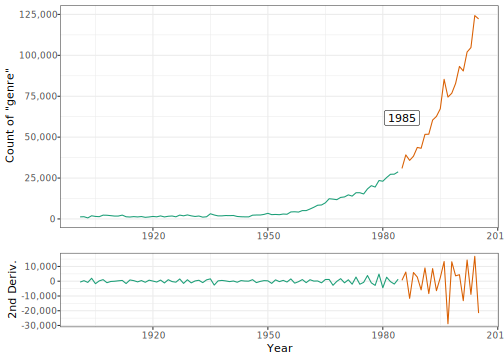
\includegraphics[width=0.9\linewidth]{ambrose_dissertation_files/figure-latex/ttsgnr-1} 

}

\caption{Absolute count of term "genre", 1901-2008. Segments correspond to significantly different second derivatives.}\label{fig:ttsgnr}
\end{figure}

Figure \ref{fig:ttsgnr2} shows a similar trend but using relative
frequencies instead of absolute counts. Here ``genre'' is plotted as its
share of all terms in the corpus. This trend exhibits no inflection
point at 1984 that is statistically significant, and visually the trend
does appear the same on both sides. No other inflections points are
detectable due likely to greater year over year variability in this
series in the first half of the century, reducing confidence in any
estimate of a change point. To interpret this difference in statistical
significance between relative and absolute measures would indicate that
interest in genre continued to grow even within a secular slow-down in
the volume of texts that resembles the familiar S-shaped diffusion
curve. Alternatively, on visual inspection of the relative curve it
appears that indeed there is an inflection point, just one a decade
later in 1996. After this point the relative frequency seems to drop
rapidly, a change that would no doubt be picked up statistically after a
few more years of data and one that may in fact be located a few years
earlier than the peak suggests. Together these trends describe a career
to the term genre that has been strong for a century and that may now be
in decline.

\begin{figure}

{\centering 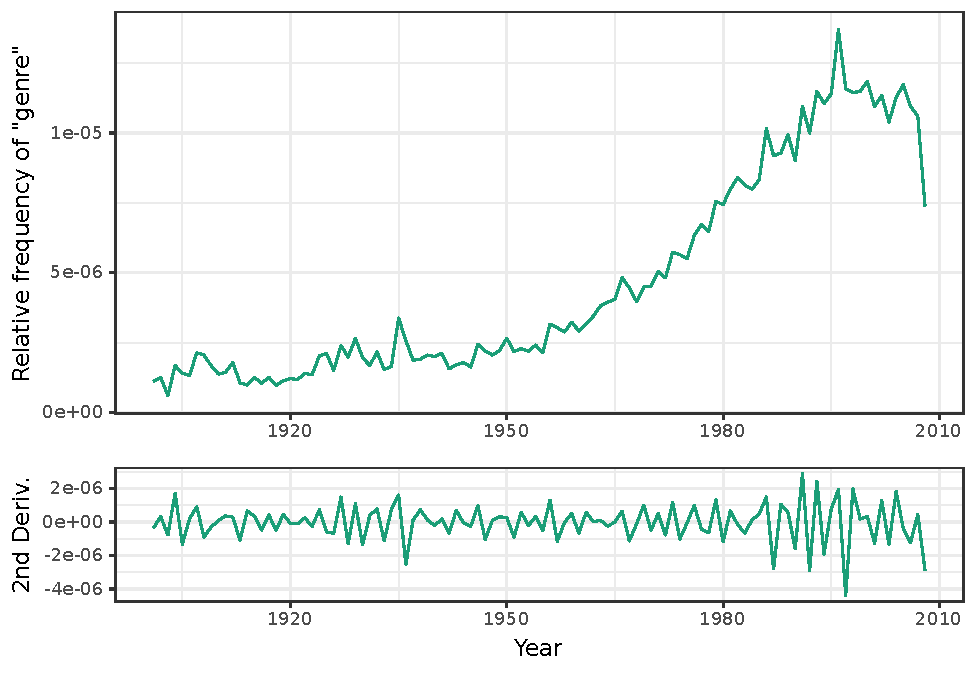
\includegraphics[width=0.9\linewidth]{ambrose_dissertation_files/figure-latex/ttsgnr2-1} 

}

\caption{Relative frequency of term "genre", 1901-2008.}\label{fig:ttsgnr2}
\end{figure}

Figure \ref{fig:genre-goog} gives an indication of what things the term
genre has been used to describe. It illustrates the frequency of terms
appearing in the Google Books Ngram corpus as the third term in the
trigrams beginning with ``genre of'' or ``genres of''
\citep{2012Google}. The size of the words is proportional to the total
frequency of the trigram in the English corpus, which spans centuries
from 1590 to 2008. The bias of the source--books--is clear in the
outsized importance of ``literature'' and ``writing'' which are followed
closely by ``music''. The next ten largest nouns are poetry, discourse,
fiction, art, autobiography, painting, film, romance, folklore, and
history. Ranked within that series would be several adjectives as well:
popular, science (fiction), historical, and literary. Each of these
terms refers to a field of concrete cultural products, with the
exception of ``discourse'' which is more abstract.

\begin{figure}

{\centering 
\includegraphics[width=0.9\linewidth]{img/genre-goog} 

}

\caption{Wordcloud of third term in 3gram beginning with "genre of".}\label{fig:genre-goog}
\end{figure}

Most items toward the top of the list are less popular (to write about)
art forms like television, dance, and theater. Toward the middle of the
list begin to appear adaptations of the term from the cultural to the
social context. These include practical fields like medicine and
journalism, political areas like law, government, and crime, and social
arenas like identity and protest.

To impose a sociological gloss on the term, these varied uses of genre
would make reviewing the literature on the topic difficult, were it not
for the discipline structure of the academy. The uses of the term genre
are themselves systematically organized by discipline, and a disciple
who is adequately trained will know the correct ways to use the term in
her local context. To use genre as a disciplinary convention means to
first identify your location in the disciplinary field, and then to
accept the limitations on scope by excluding those treatments of the
term that are extradisciplinary, that is, irrelevant. Disciplinary
structure reduces the true cultural complexity of the meaning of genre
to a restricted form, which in turn allows humble knowledge workers to
engage upon a set of shared assumptions. Such simplicity begets new
complexity as disciples spin out the consequences of their local use of
genre.

In the sociology of culture, genre is a form of classification enacted
by people in various social contexts. In the context of industrial
capitalism, genre is an economic principle helping to organize supply
and demand within markets for cultural products. There actors see genres
among the borders between economic, social, and cultural uses, as a
market category helping them acquire or produce content, as a card in
proximate games of prestige, or as something to taste, to consume and
enjoy directly. Less often genre is knowledge, a component of culture
separate from taste, that is a factor in the formation of ideas and
skills, whether these lead in turn to economic production or not.

Genre's meaning is context specific and variable across sociological
subfields, though it is amplified in empiricist fashion by economy and
society approaches that reduce genre to the act of classification
itself. I say empiricist because of the empirical ease with which the
classification or labeling actions are observed. Especially with
Internet distribution systems, it becomes trivial for corporations to
observe when a consumer labels her preferences while browsing a content
catalog; it is much harder to observe the ideas that consuming a
particular piece of content sparks in the mind.

In cultural studies genre is used much differently and much more in
accordance with its etymology. To the humanist, genre is an ontological
phenomenon, which is to say, genres are differentiated from each other
by combinations of discrete features of signs and signifieds. Humanists
are trained to establish these ontologies through methodological
readings of texts and through cultivation of theories of genre types.
These methods are at the same time empirical and interpretive, because
in consuming objective texts the researcher actually observes the ideas
that form in her own consciousness, and they may hope that others have a
resonant experience. Genres have more substance to them for humanists
than they do for sociologists. For sociologists of culture, genres are
how people use genre labels, while for humanists, genres are knowledge.

As we have said, the meaning of genre for a sociologist of culture is
economistic, at the same time a market category and a taste
configuration for consumers. The term differs for a sociologist of
knowledge, and perhaps for a cultural sociologist. It is ontology as it
is for the humanist, however it is not the ontology as represented to
the researcher in the consumption of texts. It is the hopelessly
unobservable distribution of ontologies appearing in a population of
consumers attending to similar texts. The sociologist of knowledge
accuses the sociologist of culture of reducing internalist concepts,
thought and experience, to externalist ones, taste and preference. The
sociologist of culture rejoins, show me proof, and on and on the
interlocutors spin around the axis defining the boundary between their
subfields.

But this description of subdisciplinary differences really is just an
example of a structural theory of genre that is within scope for the
sociologist of knowledge and beyond it for the sociologist of culture,
due to their epistemological differences. If genres are ontological,
then they deeply structure a person's experience of reality. Ontologies
form basic perceptual categories, and people with different ontologies
of an object experience different things even if oriented to the same
objective phenomenon. A ontological theory of genre would, for example,
attempt to explain differences in taste as differences in
phenomenological perception, whereas a taste theory of genre treats
consumption behavior as revealing preferences whose downstream
consequences are then explored.

Yet for all the differing treatments of genre mentioned above, do these
views really contradict, or are they in fact complementary? Does genre
as distribution serve the economic sociologist's goals, or does a lack
of ontological substance lead her astray? Does genre as knowledge remain
hopelessly unverifiable, or are theoretical constructs necessary to
achieve a correct interpretation of facts? Is everyone at the club
listening to the same song hearing the same thing?

\hypertarget{disciplines}{%
\subsection{Disciplines}\label{disciplines}}

To return to disciplines, answering such questions would put the
researcher in an adisciplinary predicament, for it would mean eschewing
the scope restrictions cherished by disciples. The challenges of a
meta-disciplinary analysis are manifold and uncertain. One is as likely
to grow her audience as to lose it altogether. She risks the
dilettantism of a jack-of-all-trades. What's worse, she exposes herself
to a dizzying scale of content to consider. If disciplines are indeed
functional, then the meta-analysis that effaces disciplines risks being
dysfunctional. The upside, however, is appealing. If the universe of
meanings given to the term genre does contain complementary uses, a
meta-analysis will allow one to consider the consequences of the now
arbitrary segregation of a superior metaconcept across disciplinary
boundaries. Both sides of the divide could be strengthened by a cultural
exchange of their respective terms. The redundancy of parallel discovery
can be avoided.

Pathologies of disciplinarity can be diagnosed and treated. Disciplines
are social substructures embedded in a larger society and culture.
Disciplinarity is a kind of controlled ignorance exchanged for access to
secret knowledge. The wayward uses of a term like genre are always
lurking at the edges of the firelight defined by a particular
disciplinary camp. Discipline as rigor instructs disciples to resist
flirtations with the available complexity of the term. The essential
tension is very rarely between what is known and unknown; rather it is
more commonly between what is known ``here'' versus what we are
conditioned to be willfully ignorant of ``there''.

This definition of discipline is isomorphic with that of genre, in that
disciplines are another form of categorical decision making, just at a
higher level. Disciplines are supergenres that reflect the nesting of
categories. What may distinguish them in a more serious way is the
institutional underpinning of the category. If genres are formed by the
categorical thinking of disciples, disciplines are formed by the
categorical thinking of patrons, the powerful actors like university
administrators, state legislators, and grantmakers who manage the
economic foundation of scholarly careers, as well as the elite disciples
who interface with these stakeholders. Where genre labels are inscribed
onto cultural products, texts, discipline labels are inscribed onto
cultural infrastructure like funding lines, buildings, and personnel
themselves.

In a motivation of some of the arguments to follow, I take a
metadisciplinary approach, which is to cast as wide a net as possible on
the term genre. In so doing I hope to test the tacit cultural assumption
that discipline-based decisions of relevance are valid, that is, that
when we exclude arguments from other disciplines we remove distractions
and focus on what is important. The alternative possibility is that we
are wasting intellectual resources, because to exclude important work
about our topic, even if it is codified in foreign terms, is to risk
ignorance and redundancy. The topic is genre and how disciplinary
boundaries form such that people using the same word nonetheless cannot
communicate effectively. They draw on different paradigms, which is to
say the term is not really the same term. What I hope to do is uncover
the knowledge contexts surrounding the terms, and map these contexts in
a way that enumerates the various communities of discourse and theories
constituting the term.

\hypertarget{method}{%
\section{Method}\label{method}}

As I have said, the first consequence of eschewing disciplinary
limitations is to bloat the size of the ``literature'' on genre, since
no uses of the term would be excluded. An empirical approach to the
standard academic convention of a literature review will help reign in
the scale and complexity of the task. My aim, however, remains practical
rather than scientific. The methods need to be good enough to yield
results that offer something new above a traditional literature review
relying on library search and disciplinary wisdom about what is
important. This is not because a scientific approach is undesirable, it
is that it is not yet demanded of ``the literature''. Sociologists are
not expected to take a sociological orientation toward the history of
their fields. Rather the literature review serves the social purpose of
taking a position in a field of cultural production. It is a listing of
a roster of political support and rivalry, and an advertisement to
attract a desired audience.

To take an empirical approach to the literature review would be
subversive were it not the first function of disciplinary genres to
render atypical draws from the archive irrelevant. Disciplinary
subfields, genres, are credentialed by secret sets of references, and
most comers are held at the door. This in and of itself can be
subversive of even more arbitrary club rules, namely those of
educational pedigree, such that anyone willing to invest in a
presentation of the genre definition will be granted access to the
venues, if not the invisible colleges, of the subfield. To be admitted
to the arena is no guarantee of achievement within it, but it is a
start. Nevertheless, the scale of the archive will always supply entropy
enough to create a deterrent of flotsam and jetsam around subfields
composed of projects and persons who either never cracked the code or
who willfully eschewed it.

\hypertarget{distant-sampling}{%
\subsection{Distant sampling}\label{distant-sampling}}

The research strategy here attempts to parry the entropic tendency of
the archive by substituting human for machine limits. The methodological
premise of a meta-analysis of genre is that the Gordian knot of the
global cultural complexity of the archive can be cut by stratified
sampling. I use a large digital archive of texts, JSTOR, to represent
the whole of the academic archive. Though clearly a toy representing
only a fraction of all networked scholarly produce, JSTOR is large
enough to easily surpass individual cognition and compel the equivalent
types of complexity reduction facing any researcher approaching the real
archive via their local university library portal.

I use a simple term search of the keyword ``genre'' to define half of a
sampling frame.\footnote{TODO, I did not, but should take a random draw
  of the same size to serve as a control.} I could then take a simple
random sample of texts, analyze how each uses the term genre, develop a
classification scheme, and enumerate the different uses of the term.
Unfortunately, a small sample in a statistical sense may be larger than
a poor researcher can handle. 1,000 texts is not large statistically,
but it is huge from a content analysis perspective. What's worse, 1,000
texts may still exclude, by random chance, small subcultures of the
term. Stratification within a more or less global sampling frame
resolves this issue by delineating those subcultures so none would be
left out.

Alas, the JSTOR digital archive lacks subject labels at the article
level, though it does include them for book chapters and for journals.
While not foolish, inheriting a journal label to the articles included
within it may be a coarse approximation if within-journal content
variation exceeds between-journal variation. We can use text analytic
classification methods to cluster articles directly and discover latent
groups of articles, and in so doing we can have an independent standard
to compare to the discipline labels given to journals. It is an open
question whether such methods align with what we have discussed above as
disciplinary and subdisciplinary groupings, for us whether regularities
in vocabulary correspond to regularities in the meaning of the term
genre. If they do not, then the study will only be a stop en route to a
true census of the uses of the term genre, and the contribution will be
to have interrogated the quality of the methods used, though this would
be a small consolation indeed! Even so, for a new method to claim to be
able to improve on conventional wisdom, I behoove myself to proceed
methodically.

The choice in computational text analysis (CTA) about how to represent
texts as data hinges on whether word order is preserved. The older and
more tested approach is to not preserve word order. The name given to
this ``bag of words'' format reminds one of its inelegance. A bag of
words is a frequency table for each document counting up the number of
times particular words are used, a representation that effectively
reduces a text to its vocabulary. It is the analyst's crude operational
decision to treat vocabularies as indicators of meaning, but social
scientists conventionally insist on cross validation via qualitative
analysis. While the ambitions of computational text analysis may start
with a replacement of, for instance, the standard literature review, the
conventional distrust, at least in sociology, of mathematical models of
text makes CTA more of a sampling method than an analytic method. The
study will culminate in a reading of texts, albeit one that is different
than traditional qualitative analysis because the CTA researcher
welcomes the introduction of interpretive bias from an understanding of
the mathematical model before, during, or after the texts are read. In
the game of ``choose your influence'', CTA is one choice while
disciplinary wisdom is another.

There are two types of classification methods in text analysis, direct
document clustering and topic modeling. Direct document clustering
treats the bag of words as a vector space and calculates distance or
similarity metrics between documents, which are then clustered. In a
topic model, the relationship between documents is mediated by an
unobserved but latently modeled representation of their content;
documents are similar because they are formed from the same topics.

Whichever approach one takes, and both may be used, recall that the goal
is to organize the texts into strata for the purpose of stratified
sampling. We said that we wish to typify and enumerate the different
uses of the term genre. By qualitative analysis, we could read every
text in a simple random sample and come up with a theory of the use of
genre in that text. The demerits of this approach are several
\citep[c.f.][5]{Nelson2017Computational}. It would take longer than we
want even for too small a sample. We are not humanists and have not been
trained in text analysis (this will hound us no matter what). Fatigue
will set in, and accuracy and consistency will suffer. We may limit our
set of theories to spare us the agony of complexity. It will be hard to
reproduce our results. There may be path dependency with a different
reading order producing different theories. On the upside, we would be
more educated for it.

Instead, we will stratify the sample, and it is in the configuration of
the strata that much of the work will be done. The strata impose upon
our interpretation of the texts the assumption of sameness.

\hypertarget{no-cigar}{%
\subsection{No cigar}\label{no-cigar}}

The popular yet maligned distant reading approach taken by digital
humanists \citep[e.g.~][]{Moretti2005Graphs} is being taken up with
gusto by social scientists who are less skeptical of quantitative
methods \citep[e.g.~][]{DiMaggio2013Exploiting}. Following Nelson
\citeyearpar{Nelson2017Computational} I employ a quantitative analysis
of texts not to replace human reading with machine reading but to
support reproducibility in traditional qualitative content analysis.
While CTA makes it possible to dispense with reading altogether,
knowledge, understanding, and the cultural logics of
arguments--especially their ontologies--are still only obtainable by
reading primary texts, closely or not. The most radical interpretive CTA
method would involve deep neural net supervised machine learning, which
may be able to predict how a particular human reader would classify a
text without their needing to read it, though this has never been
demonstrated. What I gain from CTA is guidance in answering the question
of what to read, and perhaps in what order to do so.

As we know, the question of what to read is answered institutionally for
scholars already by way of canon, curriculum, word of mouth, and digital
reference term search services. These are their own forms of distant
reading, because they each make obsolete the archaic image, true of
figures like Weber, of a scholar buried in library stacks reading
everything they come across (and so it has been said of Weber,
forgetting nothing).\footnote{What a scandal it would be if Weber's
  lionizers discovered that he had only read text indices! Surely they
  would bury such a fact. But the point would remain that even if a
  scholar were able to consume an entire corpus, the sheer scale of
  contemporary publication is now beyond even a genius's capacity.}
These contemporary shortcuts are historically arbitrary, but what is
important is first that they serve the function of reducing the
overwhelming cognitive complexity of published scholarship, and second
that they structure that reduction in the same way for all scholars. An
arbitrary reduction needs to be consistent to act as an infrastructure
for subdisciplinary scholarship, otherwise scholars would find
themselves located in different literatures.

If distant reading is a criticism of close reading then it has a big
hill to climb especially among humanists who are trained to deal very
carefully with texts. In the social sciences a type of customary distant
reading is that of ritual citations, those that have developed a meaning
that may be oblique to their content or at odds with the intentions of
the the original authors. A ritual citation is simply one that is cited
but not read, but also one that is so often used that its socially
acceptable usages are known from other secondary accounts. For all the
lack of due diligence in the use of ritual citations, their socially
understood meanings are better than the thoroughly perfunctory citation,
those included because they were returned by a digital reference service
and never read by anyone.

What are the social patterns of the traditional literature review are
topics for the sociology of knowledge and science and for the
information sciences. This is not the task of the current study. What we
take from the traditional approach is the consequences of excluding
large segments of intellectual history. What CTA makes possible for the
first time is a nonarbitrary, inclusive analysis of \emph{all} content
in a digitized corpus. It will not necessarily be a good analysis, but
what it will lack in quality it will make up for in coverage. A CTA
approach to the literature review will at least make clear what lacuna
would be left by the traditional approach. They also reduce the
potential idiosyncrasy of a particular author's literature review
because, unlike a personal reading, a CTA model can be communicated
precisely.

Of course the cognitive limitation of how much any scholar can actually
read and understand remains. There will be an exclusion mechanism no
matter what, therefore a chief assumption of a CTA literature review is
that corpus segmentation is both possible and that some reduced form of
reading, some sampling procedure, can be said to be representative of
the unread portion in each segment. These representative texts will be
subjected to a close reading, but their interpretation will be
generalized to unread documents. Hence I call this a ``no cigar''
approach to reading, as in ``close but''. If on the contrary to the
assumption no two snowflakes are alike, then the enterprise of knowing
more than we have before is fraught, and CTA becomes yet another
arbitrary reducer.

What is worse, or perhaps better, is that there is reason to believe
that idiosyncrasy itself is an historically variable feature of
disciplines. If institutional isomorphism has proceeded to some high
level in contemporary disciplines, then the assumption that reading the
bellwether texts is as good as reading the entire herd may hold. If this
is true, however, it raises as many questions about the process of
institutionalization in cultural production as it answers about the
potential to learn truer versions of intellectual history.

\hypertarget{topic-models}{%
\subsection{Topic Models}\label{topic-models}}

We have referred generically to computational text analysis, and now we
can discuss the topic model as our technique of choice. There are many
ways of estimating a topic model (e.g.~the famous Latent Dirichlet
Allocation (LDA) estimator) but the model itself is simple. It is a
latent variable model that decomposes a document-by-term matrix--in
which every document is represented as a frequency distribution over
every term appearing in the corpus--into two unobserved matrices:

\begin{itemize}
\tightlist
\item
  a topic-by-term matrix, and
\item
  a document-by-topic matrix.
\end{itemize}

Topics are directly represented by they topic-by-term matrix. A topic is
a probability distribution over a vocabulary. To draw on a topic means
to choose vocabulary as a random draw from this distribution, where
words with higher probabilities will be chosen more often. In the case
of genres we might imagine a topic about film and a topic about music.
Some words may be important (highly probable), to both topics, such as
the word ``genre'', while others would be distinct, such as the words
``movie'' (probable for film but improbable for music) and ``band''
(vice versa).

Note the usual distributional bait-and-switch of categorical statistical
analysis, where observed count data are operationalized as the outcomes
of unobserved probabilities. The probabilities are what will be
estimated, not the counts. The importance of this will be explored in
the sections on estimation and diagnostics, but suffice to say that the
differences between probabilities and counts encapsulate many of the
difficulties applied researchers encounter when using topic models.

Given topics as term distributions, a document can be represented not as
a distribution over terms, but as a distribution over topics. The topic
mediates the relationship between documents and terms. In order to
generate diction for a document, all that need be understood is the
ratio of topics out of which it is composed. This is sometimes explained
as a generative mechanism; to ask what word will be chosen next in
composing a document, one first samples from the document's own topic
distribution to decide which topic the word will be drawn from, and
given that topic, one then samples from the topic's word distribution to
decide which word will be included in the document. A document's topic
probabilities also create the expectation of how many words are
attributed to each topic. A document with topic probabilities .7 from
music and .3 from film would be expected to be 70 percent about music
and 30 percent about film, making for a parsimonious albeit reductive
description of document content.

It is important not to overinterpret a topic model. To describe a topic
model as ``generative'' implies that it explains how documents are
written. Such a generative metaphor reveals the absurdity of a topic
model as a representation of writing. Not to mention the fact that
punctuation tends not to be represented (though it could be), the terms
chosen would be in a random order incapable of making meaningful
sentences. Hence it is best to avoid the generative metaphor as an
explanation of texts. If topic models touch on the generation of real,
meaningful documents, it is only in a very limited sense. What the topic
model really represents is how vocabularies are organized to condition
an author's diction. A vocabulary can be thought of as an infrastructure
of meaning more trivial than grammar or syntax and much more trivial
than concepts or ideas. A topic is a simple list of words that is known
or knowable across all authors in a field. Topics do not tell stories;
authors tell stories in part by making diction choices that are
conditioned by topics.

From a sense or meaning making perspective topics are trivial; this is
because so little is known about what an author says by knowing the
topic or even the term distribution of a document. What topics are
useful for, however, is the segmentation or cartography of a corpus.
Topics are really a global feature, perhaps a cultural feature, of a
corpus of texts that is itself meaningfully selected. If indeed a field
of texts is oriented to common if not always overlapping vocabularies,
then topics can represent this well.

A topic model could be posited based on the domain knowledge of an
expert, and this would be a form of estimation. The practical value of
statistical topic modeling is that the unobserved topics can be induced,
with a raft of statistical assumptions, directly from the observed
document-by-term matrix to arrive at a model with the features just
described. An estimated topic model will contain several other
parameters filling in assumptions necessary to make it possible to
identify the unobservable topic probabilities in each of the two
matrices of the model. For instance, in LDA models the concentration
parameter commonly called alpha makes an assumption about how many
topics tend to comprise each document. Alpha values close to zero make
it very likely that documents are composed of only one topic, while an
alpha value greater than one increase the chance that a document will be
decomposed into several topics. Alpha equal to one creates no tendency,
so concentrated and diffuse mixtures are all equally likely to occur. It
would behoove a researcher to make an informed decision about this
parameter, yet software often sets an arbitrary default that the user
may or may not be fully aware of.

\hypertarget{choosing-k}{%
\subsubsection{Choosing K}\label{choosing-k}}

Finally, topic models require the analyst to choose the number of topics
K. The approach we take to guiding this decision is not to expect one
correct specification of K but rather to see it as a changing
resolution. A K=2 model usefully bifurcates the sample and is not simply
wrong because it is too restrictive. As K increases we expect the
samples to continue to divide as new parameter spaces become available
to partition the sample. While this is not strictly a hierarchical
design, since each K model is fit independently, we should expect to see
aspects of hierarchical topics as well as some degree of stability in
the relationships among topics.

Between model cross-validation means that document and term groupings
should be relatively stable as K increases. The document overlaps
between, say, a three topic model and a four topic model should not be
random. By graphing the document overlaps between pseudo hierarchically
organized models, it should be clear which topics are the most stable
and which are constituted partly by chance or by spurious association.
An ensemble approach would then recommend itself; if the content of a
topic is stable across different specifications of K, within limits,
then we should have even more confidence in that topic.

When parameter space is limited the content with the strongest signal
will come to define the topic, but the document by term vector will be
contaminated with content that would be separated given more space. For
sets of documents that are constituted by multiple true topics, we
expect to see splitting of larger topics as the resolution increases to
meet the real diversity. Hierarchy will reveal itself as topics with
stronger topic signals subsume weaker ones until K reaches a point where
there is enough space to separate them. On the other hand, in the
classic trade-off between variance and bias, where K overshoots the true
number of topics, we expect to see random splitting and possibly ``dust
bin'' effects where spare topics allow larger topics to prune their
weaker term associations. Indeed dust bins may appear even before the
true K is reached. Where the term proportions explained by topics are
very unequal, it may pay during estimation to treat a true smaller topic
as a dust bin for a larger topic, because the optiization gains of
clarifying a larger topic may be greater than the losses of confusing a
smaller one.

Another interesting feature of this approach is that it shows when and
how topics are able to appear given the parameter space constraints. We
expect the most dominant topics, those that appear at low K and remain
stable as K increases, to derive from vocabularies that are both
distinctive and used often. The content with the strongest signal will
be ``FREX'' terms, terms that are both frequent and exclusive
\citep{Bischof2012Summarizing}. Frequent means they have high counts in
the overall corpus either due to occurence across many texts or to very
large counts in a few texts. Exclusivity (or monosemy, the opposite of
polysemy) means that terms co-occur with an invariable set of additional
terms. Exclusivity is related to the notion of anchor words that are
maximally exclusive, appearing in only one topic, but likely very
infrequent.The exclusivity of terms relates to the separability of
topics \citep{Arora2018Learning}, while the topic frequency of terms
relates to the topic's contribution to explaining global corpus
frequencies, that is, to maximizing model likelihood during estimation.

It should be possible to predict a priority for topic emergence as
models increase parameter space for topics. First, we expect topic model
estimators would be very tuned to picking out even a handful of texts
written in a different language than the main corpus, as terms within
those documents would be both frequent and exclusive. We should expect
technical jargon to also send a strong signal for it's high exclusivity.
Indeed, these special vocabularies are salient for both humans and
machines for the same reason; they are easy to disassociate from the
rest of the text. The priority, however, for the estimators will be to
explain global term frequencies, so jargon will likely be behind
frequent terms that appear across multiple topics, as in the case of
polysemy or the more common case of simple language ambiguity. Trailing
the pack and the last to emerge will be, as we have discussed,
idiosyncracy.

Let us remind ourselves of what badness means, because a bad model in a
statistical sense may very well be the correct model for the analytical
purpose of the researcher. A human reader with an interpretive goal in
mind can be quite apt at scanning text content and ignoring what she
finds to be irrelevant. Some of this seeming irrelevance has to do with
the syntactic structure of language, while others a reader knows by
experience to be elements of style and rhetoric in their field. The
interpretive goal becomes like a flashlight that darkens much more
content than it illuminates.

While human readers tend to make sense of only small portions of texts,
the machine is not so lucky as to have the human capacity for selective
ignorance. The topic model estimator sees and makes sense of everything
at once. This is sometimes at cross purposes to the researcher's hope of
complexity reduction, because in interpreting the model rather than the
text she will be told by the model that something is important even if
she would have easily ignored the same context in the natural setting. A
topic model that is both correctly specified and accurately fit on a
large corpus will likely have dozens or even hundreds of topics. Such a
variegated classification scheme is likely to contain some topics that a
reader would consider to be redundant, for instance, because they are
about the same thing yet differ for an irrelevant stylistic vocabulary.
Many others will simply be irrelevant to her research agenda. The task
of sorting through the topics is supposed to be easier than sorting
through the original texts, yet the researcher is sure to find many
inscrutable lists of FREX terms in a that can only be understood with
reference to classified articles.

In the case that a correct model of vocabularly clustering is actually
too complicated to be helpful, the correct research decision may be to
deliberately underspecify the model. We can imagine the real topics as
guests standing in a line of priority, and the model is like a wedding
with a limited number of tables. The guests with the strongest relations
among them sit at the first table, the next strongest at the second and
so on until all of the tables are full. In their munificence the happy
couple still lets the remaining guests in, and what can they do but pull
up a chair at the tables where perhaps they already know one of the more
honored guests. However, if an additional table, or several, were to be
found, the crashers could look among themselves for close relationships,
even perhaps peeling away a priority guest, to form a separate group.
Prior to there being room, that group would be unrecognizably
distributed among several tables. The group would not exist, but the
individuals would, and they would find a seat somewhere.

Just as the arrival of wedding crashers at the tables does not alter the
identity of the core group that constituted them to begin with, a model
where K is set too low will serve to highlight those vocabularies that
send the strongest signals, even if the tails of these topic
distributions are contaminated by unidentified topics. From a frequency
and exclusivity standpoint the unidentified topics are the less
important ones. Smaller and less distinct groups will be occluded in an
underspecified model, and whether these are substantively important is a
theoretical decision.

\begin{table}[!htbp] \centering 
  \caption{Content priority across frequency and exclusivity} 
  \label{tab:frex} 
\begin{tabular}{@{\extracolsep{5pt}} lll} 
\\[-1.8ex]\hline 
\hline \\[-1.8ex] 
exclusivity & frequency &   \\ 
\hline \\[-1.8ex] 
  & low & high \\ 
low & 4. idiosyncrasy & 2. polysemy/ambiguity \\ 
high & 3. jargon & 1. foreign language \\ 
\hline \\[-1.8ex] 
\end{tabular} 
\end{table}

Indeed we may never expect idiosycracy to emerge as its own topic except
in the limiting case. Presumably K can be set so high as to approach the
saturation point of a topic for each document. In this event topics that
would otherwise appear in common may alter to represent the uncommon
parts of a document, and the topic would merely reproduce the term
distribution of a particular document. Thus there is a transition from
content in common to content idiosyncratic to groups of trivial size and
to individual texts in the limiting case. The model is unable to ignore
supposedly idiosyncratic content, and will thus find a way to classify
it among topics in common, effectively distorting the term vector of
those topics. There may be no objective point at which the content in
common is neatly separable from the idiosyncratic content; indeed common
content evolves only by idiosyncratic innovation. An ensemble approach
allows us to observe how particular content moves among topics as
parameter space opens up.

Finally, there may be hope that sparse model estimation techniques would
ameliorate some of the considerations above. Sparse model regulation,
such as those using the L1 or LASSO constraint, bias parameters downward
and thus may set trivial regression coefficients nearer to zero. Such an
approach may well fail to represent idiosyncracy at all, which is either
a benefit or a hazard. Such a biased model would, by effacing the
idiosyncratic portions, yield topics representing only the common
portions of documents. This avoids what we have termed contamination at
the cost of losing information that we may care about. Thus for sparse
model techniques to be used responsibly document residuals would need to
be calculated to help recover the unmodeled portions of the texts. The
model diagnostics we explore below attempt to separate model parameters
into common and idiosyncratic elements, the difference being whether the
idiosyncrasy is located in the topic model or in the residuals.

\hypertarget{bias}{%
\subsubsection{Bias}\label{bias}}

Before documenting the data preparation below, it is important to keep
in mind several sampling and modeling considerations that tend to be
overlooked. First, idiosyncrasy is assumed to be unmodelable. A flaw of
traditional topic models is that, at one level, all documents are
generic. Originality exists only in novel admixtures of vocabularies
held in common. Vocabularies that are limited to trivially small sets of
works, be they idiosyncrasies of content or style, become sources of
bias to topic model estimators. Because idiosyncratic vocabulary is by
definition rare, it lacks both the mass of frequency and distribution
across documents to be reliably picked up as a topic. Indeed, if each
document were expected to contain some idiosyncrasy, then the number of
topics needed to catch all of the idiosyncrasy would be equal to the
number of texts in the corpus. Each document would then be a combination
its own idiosyncratic topic (of which it would account for 100 percent
of topic content) and a distribution over other topics held in common.
The real number of topics would then be K+N where N is the number of
texts and practically always much greater than K. Researchers would balk
at including such a large set of extraneous topics, while estimators
would both be strained by the greater parameters space and would collide
with hyperparameters designed to militate against estimating topics
distributed only over a single document.

The impracticality from a modeling perspective of representing
idiosyncrasy coincides with the undertheorized tendency among
researchers for extreme pruning of idiosyncrasy during data preparation.
A more parsimonious modeling solution would be to allow a single extra
topic designed to catch all idiosyncrasy. Yet this would tend to violate
the assumptions behind construction of the other topics for two reasons,
first because one topic would have significant distribution across all
documents and second because terms within the topic would never be
estimated together as they would really be a mixture of N uncorrelated
subtopics.

Idiosyncrasy tends to be pruned in a desire to limit the length of the
vocabulary to bring it within the bounds of computational power and the
chances of a successful parameter optimization. Depending on the task,
however, the researcher may not be so concerned with performance, and
may leave plenty of idiosyncrasy in the sample. What then is the effect
on the topic estimation of such idiosyncrasy, since the idiosyncrasy
must end up somewhere?

First, there will be a tendency to muddy the content of common topics
with the particular idiosyncrasies of the documents that happen to draw
on them. This in part explains the long, non-zero tails of topic by term
distributions, which are usually filtered out during post-estimation and
interpretation of the models. We would however expect them to corrupt
the error structure of the topic they contaminate, leading to suboptimal
estimates of the true terms in the topic.

Second, the document proportion of the contaminated topic will be
inflated in the contaminating document. After all, the idiosyncrasy of
the document was represented, erroneously, in the contaminated topic.
Because of the length of the term vector it is not difficult to imagine
the truly pathological case wherein the probability sum of the false
portion of the topic is greater than that of the true portion. In this
event, a document could be categorized within a topic due more to the
false content than to the true content, especially if the idiosyncrasy
was placed in topics randomly. Contrary to the effect of random error in
an explanatory variable in ordinary least squares linear regression,
which is to bias the regression coefficient downward, in a topic model
the effect will be to bias the topic probability of a document upward.

\citet{DiMaggio2013Exploiting} represent a typical albeit conservative
approach to topic modeling as distant reading. Their data preparation of
a newspaper corpus about U.S. arts policy in the 1980s and 1990s
resulted in 54,982 unique terms and 7,598 documents
\citeyearpar[582]{DiMaggio2013Exploiting}. This incredible
dimensionality in the term vector, which eliminated only stopwords and a
few hand-picked terms and did no stemming, represents a very
conservative approach to term filtering admitting to no performance
based truncation. They chose a model with 12 topics. Thus in a strict
interpretation of their 12-topic model, we are to believe that the
extreme idiosyncrasy of news, with all of its historical specificity, is
contained in a noise or junk topic rather than creating bias on the
estimation of the signal topics. With such a huge term mass to classify
and so few topics in which to do it, it is incredible to think that the
algorithm would alight on a junk topic rather than using that spot for a
signal topic. It is plausible that the noise (and so offensive a term to
those reporters trying to say something new!) is distributed across
signal topics rather than being safely tossed in the dust bin. To wit,
their choice of a low alpha parameter of 0.1, which assumes that each
document is generated from relatively few topics, makes it even less
likely that the estimator would spend precious parameter space on a
noise rather than on a signal topic.

\citet{DiMaggio2013Exploiting} attempt to placate statistical criticism
by substituting quantitative, statistical forms of validation for
qualitative cross validation of topics. This may be more treacherous
than the authors admit. Their analytical approach is:

\begin{enumerate}
\def\labelenumi{\arabic{enumi}.}
\tightlist
\item
  Fit the topic model.
\item
  Sort the topic by term vectors in decreasing order.

  \begin{enumerate}
  \def\labelenumii{\alph{enumii}.}
  \tightlist
  \item
    Split the fat head from the skinny tail.
  \item
    Interpret the terms in the fat head.
  \end{enumerate}
\item
  Sort the topic by document vectors in decreasing order.

  \begin{enumerate}
  \def\labelenumii{\alph{enumii}.}
  \tightlist
  \item
    Split the fat head from the skinny tail.
  \item
    Classify those documents in the fat head according to 2.b.
  \end{enumerate}
\item
  Interpret the documents according to 3.b.
\end{enumerate}

The sorting procedures are a typical low-hanging fruit use of the model.
Even though the model is a much simpler ball of string than the original
full text corpus, it is still a very complicated statistical equation
with, in this case, 12 * 54,982 + 12 * 7,598 = 750,960 estimated
parameters. Sorting the term and document vectors allows the analyst to
proceed from an interpretation of the strongest signals toward the
weakest, stopping when the author feels satisfied that the research
question is addressed. The assumption here is that the strongest
statistical signals are unbiased, that when parameters are converted to
ranks, and the ranks are converted to truncated lists of words and
documents, that those lists are correct.

The specter that I raised above applies to the document ranking more
than to the term ranking. A formal feature of topic models is that each
topic is composed of all terms in the corpus. Of course this is an
artifact rather than an intention of the model, as the goal is to
separate relevant from irrelevant terms in the constitution of topics.
Similarly, all documents are distributions over all topics, but this is
not (necessarily) the intention; again we expect an elbow in the sorted
topic document vector in front of which are relevant and after which are
irrelevant topics. Any concentration index, such as the Gini
coefficient, calculated on the topic term and to a lesser extent the
topic document vectors will show very high concentration, where most of
the probability is owned by a few elements.

We can test for some of these expectations of bias. A document's topic
assignment may be considered suspect if its term distribution from that
topic derives from the low and long tail of the topic, rather than from
the select high probability terms normally associated with the topic's
meaning.

\hypertarget{qualitative-cross-validation}{%
\subsection{Qualitative Cross
Validation}\label{qualitative-cross-validation}}

To be sure, topic model parameters may be biased by misspecification,
and if we are being fair, by the gargantuan task we ask of them. In part
because topic models, notwithstanding their decades of development,
remain difficult to validate statistically, and in part because educated
people scoff at the idea of machine reading, many researchers ultimately
rely on qualitative interpretation to evaluate model quality. Goodness
of fit means that topics pass a sniff test upon inspection. A list of
words either does or does not inspire a theory of meaningful content,
and this theory either is or is not confirmed upon inspection of
document with a highly ranked topic probability.

The same scholars who promote qualitative cross validation (QCV) would
presumably have bet on John Henry rather than the steam drill. The
arguments against the machine, which excels only at recognition, is that
it is a ham-fisted intruder into the delicacies of sensemaking,
semantics, and interpretation. Meaning operates very differently from
information namely by bringing grounding to the response to information.
One example of grounding is spreading activation, that when information
is presented to the mind by sensation, the mind responds by representing
not only a construct of the stimulus but also a network of constructs
adjacent in memory to the stimulus. Simply, humans see more than they
perceive, but machines cannot.

That machines are dumb because they recognize rather than interpret is
not entirely fair. In machine learning the analog to memory, be it
treated as semantic grounding or anything else, is mathematical model
representation, and the analog to learning is a Bayesian updating of old
models with new data. A machine seeing new data with an old model can
indeed see more than it perceives. At this moment in the era of
computational social science, however, researchers train models for the
first time on the data they wish to explain. It is theoretically
possible to communicate and transport models from past to present
researchers, however this is not done in practice for lack of
infrastructure and more importantly because social scientists rarely
study the same thing twice. Where data are ample it is possible to
simulate a history of memory for the machine using hold out techniques
where a model is trained on one sample of the data and applied to
predict another sample. Where the goal is to maximize prediction,
training and hold out samples are randomly selected. A different
approach \citep[e.g.~][]{Nay2017Predicting} involves selecting training
and hold out as a process in time. This is a closer approximation to
human memory, as humans always approach the present only armed with a
memory of the past. In this sense a time ordered model training process
may create the same kind of errors on new data that a social institution
would.

As clever as the time sorted hold out strategy is, it is unlikely to
outperform a supervised approach to model validation wherein human
judgements serve either as diagnostics or training materials for model
fitting. Human culture is far too expansive to be modeled by a computer
for no simpler reason than the data of human memory are always rapidly
lost and what is retained is selected for arbitrary historical reasons.
What makes the contest between John Henry and the steam drill
interesting in the modern era is the social problem of cultural
reproduction. Machines will outperform humans only where human history
is made more accessible to machines than to humans, which may be a join
function of the success of digital archiving coupled with the
deterioration of human education.

In the case of topic models, some advocates for the machine go so far as
to claim that the topic model actually recovers semantic context
\citep[578]{DiMaggio2013Exploiting} or what we have called grounding.
Semantic context is a more specialized notion than memory, and it refers
to the human capacity for reproducing common meaning. In language viewed
through a topic model a large collection of terms defines the topic
while only a sample of these terms will be observed in a particular
document. In this sense the topic model fills in missing information in
the way that meaningful interpretation does. This notion rests on a very
strong assumption, however, which is that information tacit in a
particular case is explicit in a different case, indeed a quorum of
different cases, and that the cases overlap enough to become included
under the same topic. With big variation in document length topic models
may take grounding, which is properly a community resource, arbitrarily
from the longer documents within a corpus thus giving them undue
influence over sensemaking. In real sociocultural interaction, a large,
exogenous influx of novel term associations would not determine meaning
at the margin. Real meaning has legitimacy enforced by interested
actors, such that deviant term associations are negatively sanctioned.
Topic models only learn from cultural expression and are ignorant of
social processes that condition expression. If novel terms are
associated in one text with a core of common terms found in many texts,
they too will be added to the topic. This is a corruption of the
grounding that would not occur in real life.

The estimation of grounding would seem to compete against the other
feature of polysemy, that a term may appear in multiple topics each with
a different context. How does the machine know that a particular term
distribution (document) is a case of missing grounding within the same
topic as another document, or is in fact a different topic with a
different context? Of course the machine knows nothing other than how to
maximize an objective function. Estimators are designed to start from a
more or less arbitrary guess and update parameters in the direction of
models that are more likely given the data. Indeed, it is the
hyperparameter choices of the researcher that often decide which
research approaches will win out. For example, the question of whether
or not a topic model detects polysemy is operationalized as topic
correlation and governed by the choice of the sigma prior, which
controls the diagonalization of the correlation matrix, where a
constraint toward low topic correlations prohibits detection of
polysemy. The current state of software discourages an understanding of
how hyperparameter tuning relates to a particular research agenda, and
this opacity to the method is a strong driver toward QCV.

Cheap computing does make grid searching across hyperparameter settings
possible, if not cost effective, but until this approach is usefully
automated it is safe to assume that models will be misspecified in an
unknown way, that the model is tuned in a particular arbitrary
theoretical direction that is unknown to the researcher. Why would one
believe that QCV would inoculate against the hidden bias imposed by the
model? To be clear, a biased model is one that will present a vocabulary
that \emph{does not} represent the text accurately. In the conventional
use of topic models, the researcher is eager to use the topic as a lens
that both arranges documents into relevant subsets (a particular draw
from the archive) and primes her interpretation of the documents content
by a suggestive list of terms. We wish to keep two forms of QVC error in
mind.

The first is classification error. Continuous document by topic
probabilities are interpreted categorically according to an explicit or
tacit threshold of classification. Explicitly, one could analyze the
global decay of topic probabilities and attempt to find natural
empirical separations at threshold values. More commonly, the tacit
satisficing criterion is met as one walks down the ranked list of
documents and eventually decides that they have understood the topic.
The error arises in the within-class generalization where classification
quality has degraded in a continuous fashion (and past the point reached
by our satisficed reader) yet such errors have been effaced by the hard
classification rule. In short, by understanding the bellwethers, the
researcher only partially understands the corpus and indeed only further
mystifies the poorly classified stragglers.

It will help to visualize the statistical situation leading to this
error. In the expected case of model misspecification, usually too few
topics, we should also expect an urchin shaped quality distribution
where on each topic spine are bellwether documents drawn out by their
strong signal to be representative of the topic. As one descends the
spine of each topic we will begin finding the poorly classified
documents collected on the body of the urchin. These documents are
representative of no topics, that is, equally representative of all or
several topics. For a misspecified model, it is possible that a
collection of these stragglers would be given a home in a model with an
extra spine, that is, new parameter space for an extra topic. But
without a topic to represent them, the analyst may make the mistake of a
false generalization from bellwether to straggler documents. Such
stragglers may even be halfway up the spine, assuring their
classification but for the wrong reason: bellwether documents achieve
their topic probability by virtue of words at the head of the sorted
topic by term vector, whereas stragglers achieve their lesser but still
above threshold topic probabilities from the meaningless long tail of
the topic by term vector. This long tail, we must recall, contains terms
that may have trivially small topic probabilities when considered
separately, but when considered together, because the term vector is so
long, their cumulative probability of the false segment of the vector
may rival in classification power that of the true segment.

The second is confirmation bias. Readers tend to skim and scan documents
more quickly and less carefully when they are told what they are about
ahead of time. It is natural for researchers to want to examine the
document by term vectors of the topics in order to understand the
results of the model and apply the findings to solve research problems.
These lists may be very evocative of theoretical assumptions and
practical expectations about the corpus, which has not normally been
read ahead of time. Theories of the meaning of the term lists are very
likely to establish confirmation bias in the reading of the texts. This
means that documents that have been classified by a satisficing or
threshold rule will be read differently with a theory of the topic in
mind than they would have otherwise. Confirmation bias means that the
analyst will have a tendency to focus on content that appears to conform
to the topic theory while discounting content that contradicts it.
Sometimes this will be warranted; after all, a feature of the model is
the ability to classify documents into multiple topics. In the
pathological case, however, the meaning of the document will be
distorted to fit the theory of the topic. A model that causes the reader
to misread a document is certainly not helpful, and the pull of
confirmation bias tends to be strong even when one is aware of it.

Fortunately we may adjust our research strategy to avoid each of these
errors. First, to ameliorate the effects of misclassification, a simple
concentration metric such as the Gini coefficient applied to the vector
will help discriminate between documents classified strongly into only a
few topics (highly concentrated probabilities) from documents that are
classified weakly into all (that is none) of the topics (unconcentrated
probabilities). To assess a particular topic classification it should be
possible to decompose the portion of a document's text that is estimated
to derive from a particular topic. That portion can then be scored
according to its weighted average rank of the terms actually contained
in the document, with poorly classified texts having lower scores. The
utility of this quality scoring is to shine a light on the yet to be
correctly classified texts, which may give an indication of when it is
warranted to increase the parameter space of the model, and which may
substantively reveal the less dominant (perhaps dominated) vocabularies.

Second, it is a simple enough procedure to forestall interpretation of
the topic by term vectors until after a direct inspection of documents
grouped by their topic classification. Indeed, this may promote a more
accurate theory of the topic since terms will be interpreted within
context.

\hypertarget{data}{%
\section{Data}\label{data}}

The JSTOR Data for Research service allows researchers to download
non-consumable versions of full text in very large samples up to 25,000
documents. We will use the JSTOR Data for Research service to download a
bag-of-words text corpus for topic modeling. I take the following steps
to develop a corpus:

\begin{enumerate}
\def\labelenumi{\arabic{enumi}.}
\tightlist
\item
  Search dfr.jstor.org using the query
  \texttt{(ta:genr*\ OR\ ab:genr*)\ AND\ la:eng} and requesting 1grams.
\item
  To cull documents for which genre is not an important term, exclude
  documents containing fewer than five variants of the term genre
  (1grams matching the regular expression \texttt{\^{}genr}: genre,
  genred, and genres).
\item
  Remove 1grams appearing fewer than three times, which often includes
  optical character recognition errors.
\item
  Remove 1grams shorter than three characters and longer than 25
  characters, again often OCR errors but also stopwords that will be
  removed anyway.\footnote{The Freudian ``id'' is an unfortunate
    casualty of this step, as well as some footnotes, endnotes, and
    captions containing small text where word boundaries were not
    detected during OCR and a series of words was concatenated.}
\item
  Remove 1grams longer than three characters that are all the same
  letter, often OCR errors but sometimes real, as in Roman numerals.
\item
  Compile baseline word counts for each document assuming that at this
  step the documents contain only valid terms, and no OCR errors.
\item
  Remove SMART stopwords.
\item
  Remove numbers.
\item
  Remove punctuation, except intraword hyphens.
\item
  Lemmatize or stem English words.
\item
  Remove lemma with fewer than three characters.
\item
  Aggregate 1grams defined by a single lemma and, for ease of
  interpretation, name the sum after the most common 1gram.
\item
  Remove terms appearing in fewer than 20 documents.
\item
  Remove documents that, after the above filters, have a word count of
  fewer than 500 words.
\item
  Remove documents that are identical in content to another document
  even if metadata differ, i.e.~reprints.
\end{enumerate}

The initial query returned 7,695 articles from 1,205 different journals,
as well as 6,485 book chapters from 4,427 books. After the above
processing steps, the sample was reduced to 3,547 articles and 2,797
chapters, or 6,344 total texts.

It is fair to ask what is lost during the pre-processing of texts. Many
are included in error due to JSTOR's internal translation of abstracts;
where ``genre'' is the French translation of the English ``kind'' the
text will be included even if the term genre does not actually appear in
the English title or abstract. While I do not carefully look at the
content of the excluded documents, assuming they were not texts that
made important use of the term genre, I do retain some information about
what components of a text were lost of those documents that were not
cut. This is a measure I call idiosyncrasy, or the proportion of terms
in a document eliminated during pre-processing. I call it idiosyncrasy
because the pre-processing condition was that terms would be eliminated
if they did not appear in at least 20 other texts. Texts that lost a
large volume of words to this filter are drawing on a vocabulary that
almost no other texts use. It would not be surprising if these were
ethnographic or content analytic studies of non English materials.

Figure \ref{fig:idi-hist} shows the right-skewed distribution of
idiosyncrasy. The median text lost about one tenth (10.19 percent) of
its words, while 90 percent of texts are within two tenths, and outliers
begin at about three tenths as can be seen in the boxplot. The 153 (2.41
percent of) texts above three tenths vary across a range as wide as the
rest of the distribution. The most idiosyncratic text, at 60.4 percent
of its vocabulary lost, is Welsh's ``Editorial: The Genre
Revival''.\footnote{www.jstor.org/stable/10.2307/27909026} The article,
from the journal \emph{Hebrew Studies}, is a single page introduction in
English to a 12 page essay reprinted in the original Hebrew. By page
count alone we would expect the idiosyncrasy to be 12/13 or 92.3
percent, which also illustrates how terms that are not in the Roman
alphabet may be discarded as OCR errors even prior to the idiosyncrasy
measurement.

\begin{figure}

{\centering 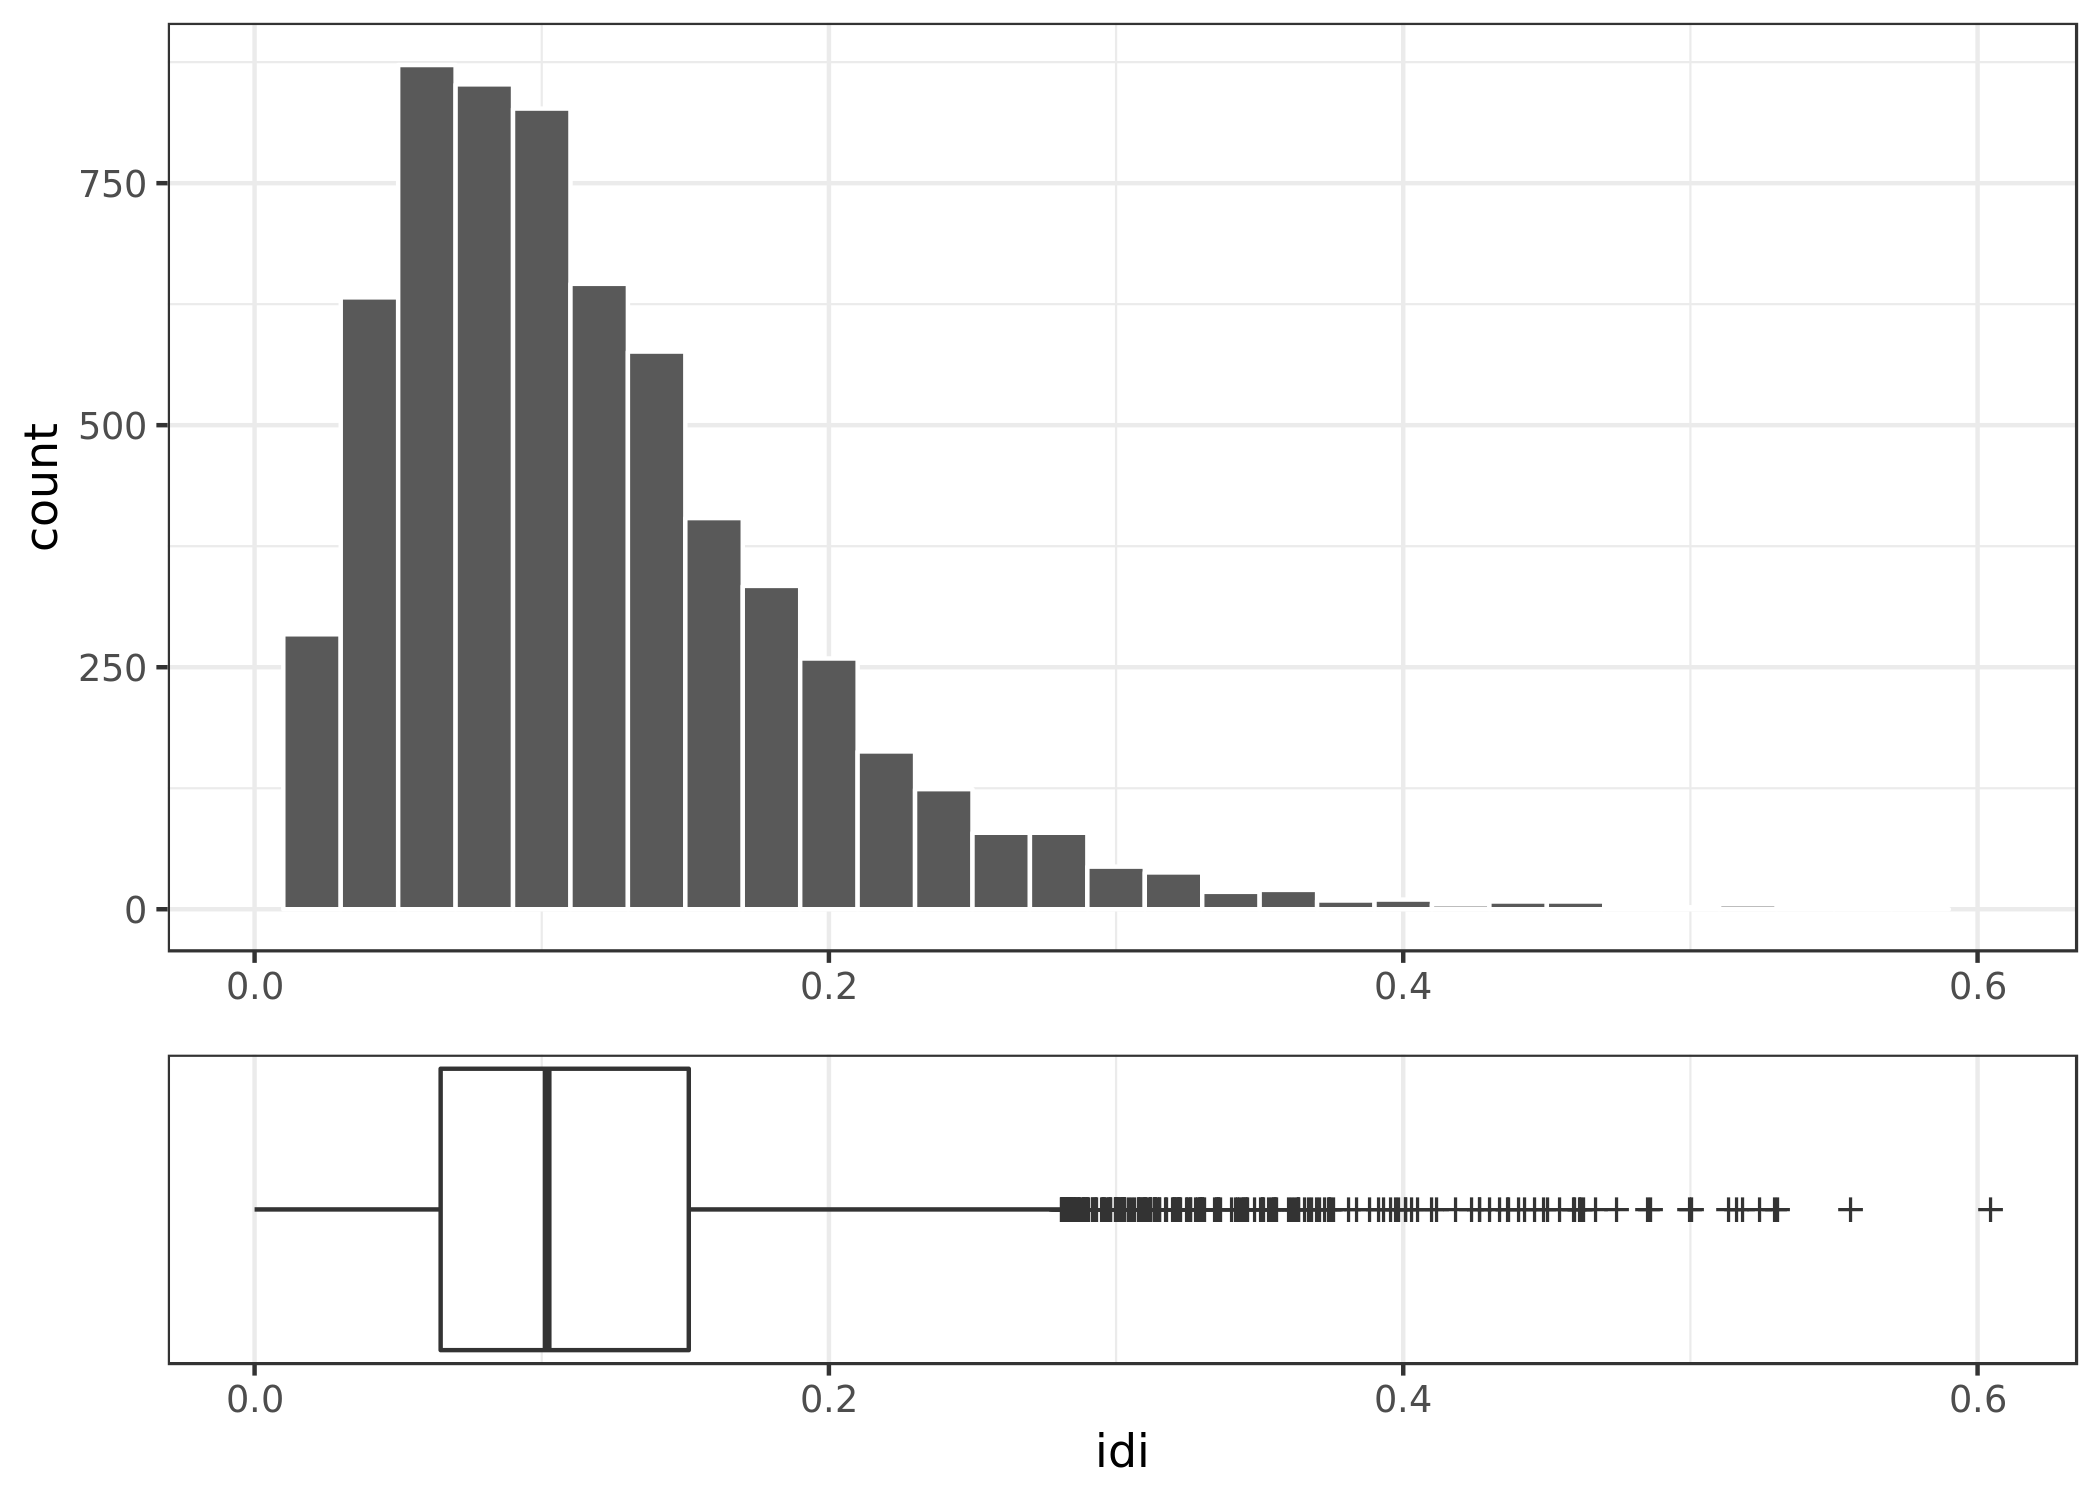
\includegraphics[width=0.9\linewidth]{ambrose_dissertation_files/figure-latex/idi-hist-1} 

}

\caption{Distribution of idiosyncracy, the proportion of document vocabularly dropped during pre-processing. Pluses indicate outliers.}\label{fig:idi-hist}
\end{figure}

Figure \ref{fig:gp-hist} shows the logarithm of the count of the term
genre as a proportion of the total term count of a text. This
distribution is much more highly skewed but contains fewer outliers. In
the median text a genre variant accounted for about 6 in 1,000 terms,
while at the 90th percentile the rate is 27 in 1,000. 44 texts (0.69
percent) are outliers where one in ten or more words is a genre variant.
The text with the largest genre proportion, at 35.7 percent of its
words, is Welsh's ``Editorial: The Genre Revival''\footnote{www.jstor.org/stable/10.2307/43795866},
a single page introduction in a special issue of \emph{Literature/Film
Quarterly} on genres.

\begin{figure}

{\centering 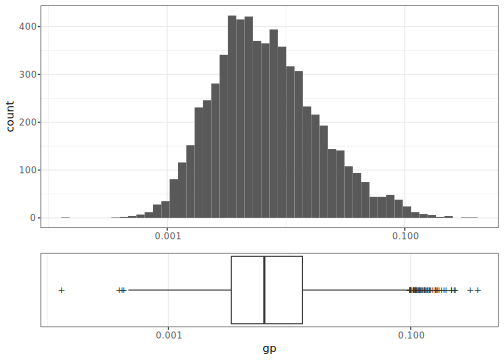
\includegraphics[width=0.9\linewidth]{ambrose_dissertation_files/figure-latex/gp-hist-1} 

}

\caption{Distribution of $log_{10}$ of the count of the term "genre" as a proportion of all terms in a text. Pluses indicate outliers.}\label{fig:gp-hist}
\end{figure}

\begin{table}[!htbp] \centering 
  \caption{Subject Distribution of Texts} 
  \label{tab:genre-jsubj} 
\begin{tabular}{@{\extracolsep{5pt}} lrrrr} 
\\[-1.8ex]\hline 
\hline \\[-1.8ex] 
Subject & N Percent & W Percent & N Rank & W Rank \\ 
\hline \\[-1.8ex] 
Language \& Literature & 20.29 & 26.96 & 1 & 1 \\ 
Humanities & 13.45 & 11.5 & 2 & 2 \\ 
History & 8.77 & 8.56 & 3 & 3 \\ 
Social Sciences & 7.19 & 5.46 & 4 & 7 \\ 
Area Studies & 5.57 & 3.55 & 5 & 6 \\ 
Sociology & 4.72 & 5.57 & 6 & 4 \\ 
Film Studies & 4.02 & 6.09 & 7 & 8 \\ 
Music & 3.83 & 4.84 & 8 & 5 \\ 
Arts & 3.65 & 3.33 & 9 & 9 \\ 
Education & 2.89 & 2.39 & 10 & 11 \\ 
Religion & 2.64 & 3.06 & 11 & 10 \\ 
Anthropology & 2.06 & 1.87 & 12 & 13 \\ 
Art \& Art History & 1.95 & 2.17 & 13 & 12 \\ 
Asian Studies & 1.77 & 1.18 & 14 & 15 \\ 
Performing Arts & 1.55 & 1.71 & 15 & 17 \\ 
Linguistics & 1.46 & 1.2 & 16 & 16 \\ 
Philosophy & 1.2 & 1.24 & 17 & 14 \\ 
Middle East Studies & 1.02 & 0.65 & 18 & 19 \\ 
Political Science & 1 & 0.88 & 19 & 21 \\ 
Other & 10.98 & 7.79 &  &  \\ 
Total & 100.02 & 100.01 &  &  \\ 
\hline \\[-1.8ex] 
\end{tabular} 
\end{table}

Table \ref{tab:genre-jsubj} enumerates the subject labels each text
inherits from its parent book or journal. JSTOR categorizes the volume
rather than each item of its contents, and volumes may bear multiple
labels. The count (N) of discrete labels as a percentage is listed first
and the table is sorted by that figure. In addition, to prevent double
counting of texts bearing multiple labels, each label is given a weight
(W) that is the inverse of the number of labels given to the text. The
top three, Language \& Literature, Humanities, and History, are the same
in each case, while Sociology, Music, and Area Studies are ranked higher
by weight than by count, an indication that Social Sciences frequently
co-occurs with other labels and is therefore down-weighted. This makes
sense as Social Sciences, like Humanities and Arts, is a meta subject.

``Subject'' is the name given by JSTOR as a description of content, yet
they also refer to ``discipline'', which as mentioned above is a
description of conditioning social structures. This is not a mere
mincing of words; the argument is that content and condition are related
but not equivalent, that is, that \emph{some} cultural formations
(topics) will span social boundaries. These rankings, especially the
lopsided proportion allocated to Language \& Literature, provide
expectations as to the number and content of topics, under the
assumption that there is less within discipline than between discipline
variation in vocabulary. Of course the goal is not to merely recover
these discipline categories which are already given. Rather, the aim is
to drill down to regularities of speech as indicators of a freely
variable cultural dimension that is conditioned but not entirely
controlled by social structure.

\hypertarget{estimation}{%
\section{Estimation}\label{estimation}}

I will I use the \texttt{stm} package in R to estimate a series of topic
models \citep{Roberts2013structural, Roberts2018stm}. The structural
topic model (STM) is a variation on the correlated topic model (CTM)
that allows for direct estimation of how covariates affect topic
formation. The CTM was an early modification of the initial latent
Dirichilet allocation (LDA) estimator, which tended to create topics
that were statistically independent of each other and which therefore
made it difficult to model documents as composed of multiple topics, a
feature which has become central to the usefuleness of topic models for
applied research \citep{Blei2007correlated}. It will be helpful to
understand the complexity of the CTM before complicating it further,
thus for the sake of simplicity we use the \texttt{stm} package to fit
CTMs without leveraging the additional feature of covariate modeling.

To briefly explain the difference, the STM builds on the CTM by modeling
the effect of document level covariates on topics in two different ways.
First, covariates may affect topic prevalence. For example, including a
dummy variable for the JSTOR discipline label Social Science interacted
across all topic by document probabilities would provide a parameter
measuring the degree to which social science texts contribute terms more
or less frequently to that topic than do non social science texts. For
example, a binary category between social sciences and humanities
interacted with a topic about music might show that social science texts
are ten percent less prevalent in the music topic than are humanities
texts. Second, covariates may affect topic content. Here the terms of a
document inherit the covariate assigned to their document of origin. A
social science dummy interacted across all topic by term probabilities
provides a parameter measuring the degree to which a term of a
particular covariate origin is more or less likely to contribute to a
topic. In practice, content models help construct two different term
rankings for the same topic, two because estimation on the high
dimensional term vector space is intractable for all but the simplest
binary covariate. In the same social science versus humanities binary,
the content model would show how the vocabulary of social science texts
differs from the vocabulary of humanities texts when talking about the
same topic, music. In a subsequent chapter we will find occasion to use
these more powerful features of the STM.

Because there are so many parameters CTM models are difficult to
estimate, but the core approach is the familiar maximum likelihood
framework. Estimators attempt to discover the parameters for the
unobserved portions of the model that are most likely given the observed
portions, the document by term counts. The estimator used in the stm
package is a version of expectation maximization (EM) in which some
parameters of the model are set arbitrarily, for instance randomly, in
order to reduce the likelihood function to something tractable that can
be maximized. The outcomes to each step of this expectation (guessing)
and maximization (solving) procedure are then fed into another
interation. In practice each step of guessing leads to a smaller change
in the parameters, and the model is said to have converged when the
changes fall below a predetermined threshold.

The parameter space of topic models is far too complex to be able to
write solveable likelihood equations and even for EM estimators to guess
at them with consistent and accurate results, so topic models frequently
include a raft of simplifying hyperparameters to reduce the
dimensionality of the problem. It is not within the present scope to
discuss these hyperparameters unless they are exogenous and can be set
in ways that are practically meaningful for applied research problems.
We have already discussed two of these, the alpha and sigma priors,
which let us control the level of mixture of topics within documents and
the correlation of topics respectively. We trust that others that are
endogenous to model estimation lead to sensible results.

Hyperparameters aside, it is also necessary to initialize the
substantive parameters of the model for the first EM step. The choice of
model initialization is substantively meaningful and under the user's
control in the stm package. For example, the CTM model may be
initialized with the values of an LDA model where topics are
uncorrelated; in this situation EM would step the topic by document
probabilities toward a more correlated outcome in which certain topics
appear together frequently, if this model is more likely given the data.

The initialization we will use is called spectral initialization, which
is related to the concept of anchor words discussed above. A spectral
model considers only the square term by term matrix where each column
and row refers to the number of times a particular word co-occurs within
any document with every other word in the vocabulary. A dimensionality
reduction technique such as principle component analysis or matrix
factorization can be used to represent each term in a number of
dimensions equal to the desired number of topics. This can in turn be
used to initialize the topic by term matrix of the model. Finally, the
usually much simpler topic by document matrix can converge quickly using
EM on the basis of the good guess supplied by the spectral model.

Because the vocabulary vector tends to be very long it is not trivial
even for spectral methods to reduce the term by term matrix to the
number of topics without additional assumptions.
\citet{Arora2018Learning} have shown that assuming the existence of
anchor words makes the decomposition fast and efficient while retaining
the feature of a single determinate solution
\citep{Roberts2016Navigating}. An anchor word is one whose probability
is one for one topic and zero for all others. In the space of the
solution the anchor words become the farthest corners of the
multidimensional cloud of terms, and a convex hull drawn through them
will contain all other terms. If the anchors are treated as singularly
representing their entire topic, the position of every other term can be
represented as a linear combination of the positions of all the anchors.
The linear weights of the anchors then become the topic probabilities of
the words, such that the closer a term is to an anchor the higher its
probability from the anchor's topic and the lower the probability for
all other anchors' topics. An anchor for each topic must be annointed so
that its vector can be set to the assumed maximum sparsity, and the
criterion for doing so is to find words with the above mentioned maximum
frequency and exclusivity, words that always appear only given a
particular set of other words. Even if the anchor word assumption is not
strictly valid, using an anchor based spectral initialization in
combination with the EM estimator may relax the assumption of sparsity
(monosemy) and allow some distribution of erstwhile anchor words
(polysemy) among topics.

Above we commented that sparse model techniques like L1 regularization
could help clarify topics by setting more coefficients to zero. Such
techniques create biased models in that they are less likely given the
data, but the hope is that in the case of topic models it is the
irrelevant terms of a topic or topics of a document that will be biased
downward, in essence making regularization a kind of filter on the
idiosyncratic portions of the corpus. Unfortunately, this desireable
filter may not be the actual effect of regularization. Sparse model
techniques tend to bias downward the coefficients of terms that are
highly correlated with other terms that themselves have a stronger
association with the outcome. By assigning the portion of variance
explained that overlaps among correlated predictors to the stronger
term, it resolves an intractable ambiguity in an arbitrary way. In this
situation L1 regularization may, in the topic by term matrix, occlude
important and relevant terms rather than prune irrelevant ones, such as
idiosyncratic or suppressed topic terms. This may actually make it
harder to interpret topics without helping resolve topic corruption.

In the document by topic matrix L1 regularization may be more helpful by
leading to topic concentration, which creates an effect similar to
setting the alpha concentration parameter of the Dirichilet distribution
in LDA below one. Like a short blanket that cannot keep the head and
feet warm at once, regularization may also offset the goal of modeling
topic correlation introduced by the CTM. There is no statistical guide
out of this morass. The impractical solution is to fit models under
multiple assumptions and compare the results by QCV. For a model that is
already as complicated to interpret as the topic model, this would be a
steep climb for most researchers. The normal remedy is liberal use of
George Box's assertion that ``all {[}models{]} are wrong''
\citep[582]{DiMaggio2013Exploiting}, which may not satisfy those hoping
that topic models can shed light on the more easily occluded corners of
intellectual history.

Notwithstanding the deep inventory of research decisions we have
mentioned, will begin with the conventional hyperparameter assumption of
the number of topics K. We fit nine models in sequence from K = 2 to K =
10 in order to use the development of topics through the K space as
context for the interpretation of the focal ten topic model. We set the
sigma prior to zero to allow for the free estimation of document by
topic correlations, which can be set as high as one to mitigate the CTM.
We use spectral initialization, which we recall relies on the anchor
words assumption to facilitate a determinate solution the topic by term
matrix that is then updated to find a more likely within document topic
mixture. In spectral initialization there is no alpha concentration
parameter as in LDA, and because we do not use L1 regularization we
create no preference during estimation for sparse, concentrated document
by topic distributions. These choices favor a less biased and more
saturated model.

To set up QCV prior to model inspection, we use the document by topic
matrix of the focal ten topic model to establish a sampling frame for
the creation of test comparisons. These comparisons are designed to
establish the presumptive substantive validity of the head of the
document by topic probabilities without consideration of pathologies
arising from tail-based classification errors. In these ``sniff tests'',
which are explained in greater detail below, I ask myself to recover
model classifications of documents by inspecting selected documents
without prior knowledge of topic by term content. While this is an
admittedly seat-of-the-pants goodness of fit test, if I cannot make
sense of topic separation then there is a more serious problem with the
core deliverable of the topic model. Passing these tests is a necessary
check before getting into more subtle model interpretation concerns.

\hypertarget{diagnostics}{%
\section{Diagnostics}\label{diagnostics}}

Having fit nine models sequentially from K = 2 to K = 10, we alight on
the final as the focal model given that we assume that at ten topics we
have still underspecified K. In this section I implement the several
approaches to validating topic quality mentioned above. Some diagnostics
use measures calculated on the first eight models to contextualize the
ninth, while others are perfomed only on the focal model. These are
necessary guides to interpreting topic models as a form of analysis
whose final results are almost guaranteed to be misspecified. Diagnostic
procedures help to avoid mistakes in interpreting a bad model. If all
models are wrong, then it behooves us to always interpret model results
in the context of diagnostics.

\hypertarget{ghost-probability}{%
\subsection{Ghost probability}\label{ghost-probability}}

Ghost probabilities are terms that are expected to be but are not
actually present in a document. By the logic of the topic model these
occur because documents draw on only partially overlapping vocabularies;
those parts of the vocabulary that do not overlap will still be assigned
to the topic and will be present only in some documents. These may well
include idiosyncratic terms, in which case they represent a bad fit. If
they are taken as valid then they imply that if a document were to be
written again, or to continue to be written, then eventually these terms
would show up. Indeed we expect the proportion of ghost terms to be
higher the shorter the document, even when the topic in which it is
classified is well behaved. In the spreading activation theory briefly
mentioned above, to the extent that topics can be thought of as a
meaningful grounding that helps to control both the generation and
interpretation of texts, then it is possible that the reading of a
document containing only a portion of the topic will elicit or bring
close to the mind terms that are not actually present. If the grounding
is expected to be corrupted, for instance with the idiosyncracies of
very long documents, then ghost terms are a source of bias. So ghost
terms are either a feature or a bug depending on how the topic model is
itself reified.

The sum of ghost term probabilities by document ranges from only a few
(14 percent) to almost all (98 percent) of the words predicted to be in
a text. The mean and median are 68 percent and the distribution is very
close to being normally distributed notwithstanding its bounding between
zero and one. Figure \ref{fig:ghostN} shows that, predictably, the
proportion of ghost terms is strongly associated with document length.
Predicting the log-odds of the probability makes for a better fit for
the smallest documents (as illustrated), but for the sake of simplicity
in the bulk of documents between 100 and 1,000 words in length, the
association of the untransformed probability with the \(log_{10}\) of
document length is linear, with a ten percent increase in length
associated with a one-third (0.346) decline in the ghost probability.

In a topic model every document is predicted to be a distribution across
the entire corpus. The fewer the number of words in the text, the more
it will be predicted to contain words not appearing in the original.
From the model perspective a small text, like any small sample, will be
expected to have high variance across multiple draws. This implies that
the particular instantiation of the text is arbitrary. Another way to
say this is that the grounding of smaller texts is much more important
than for larger texts, since there are many more blanks to be filled in.
The uncertainty around small texts from a statistical perspective
inverts the usual sense that a reader has that a smaller portion of text
is easier, not harder, to understand, or from the writer's perspective,
that brevity is the soul of wit. Of course such ease would derive from
the quality of the reader's own grounding; short texts never seen before
may be difficult for both human and machine alike to classify because
they lack the length to disambiguate the proper grounding. In any event
readers using a topic model to understand short texts should question
whether the model's best guess is indeed the proper semantic context for
interpretation.

\begin{figure}

{\centering 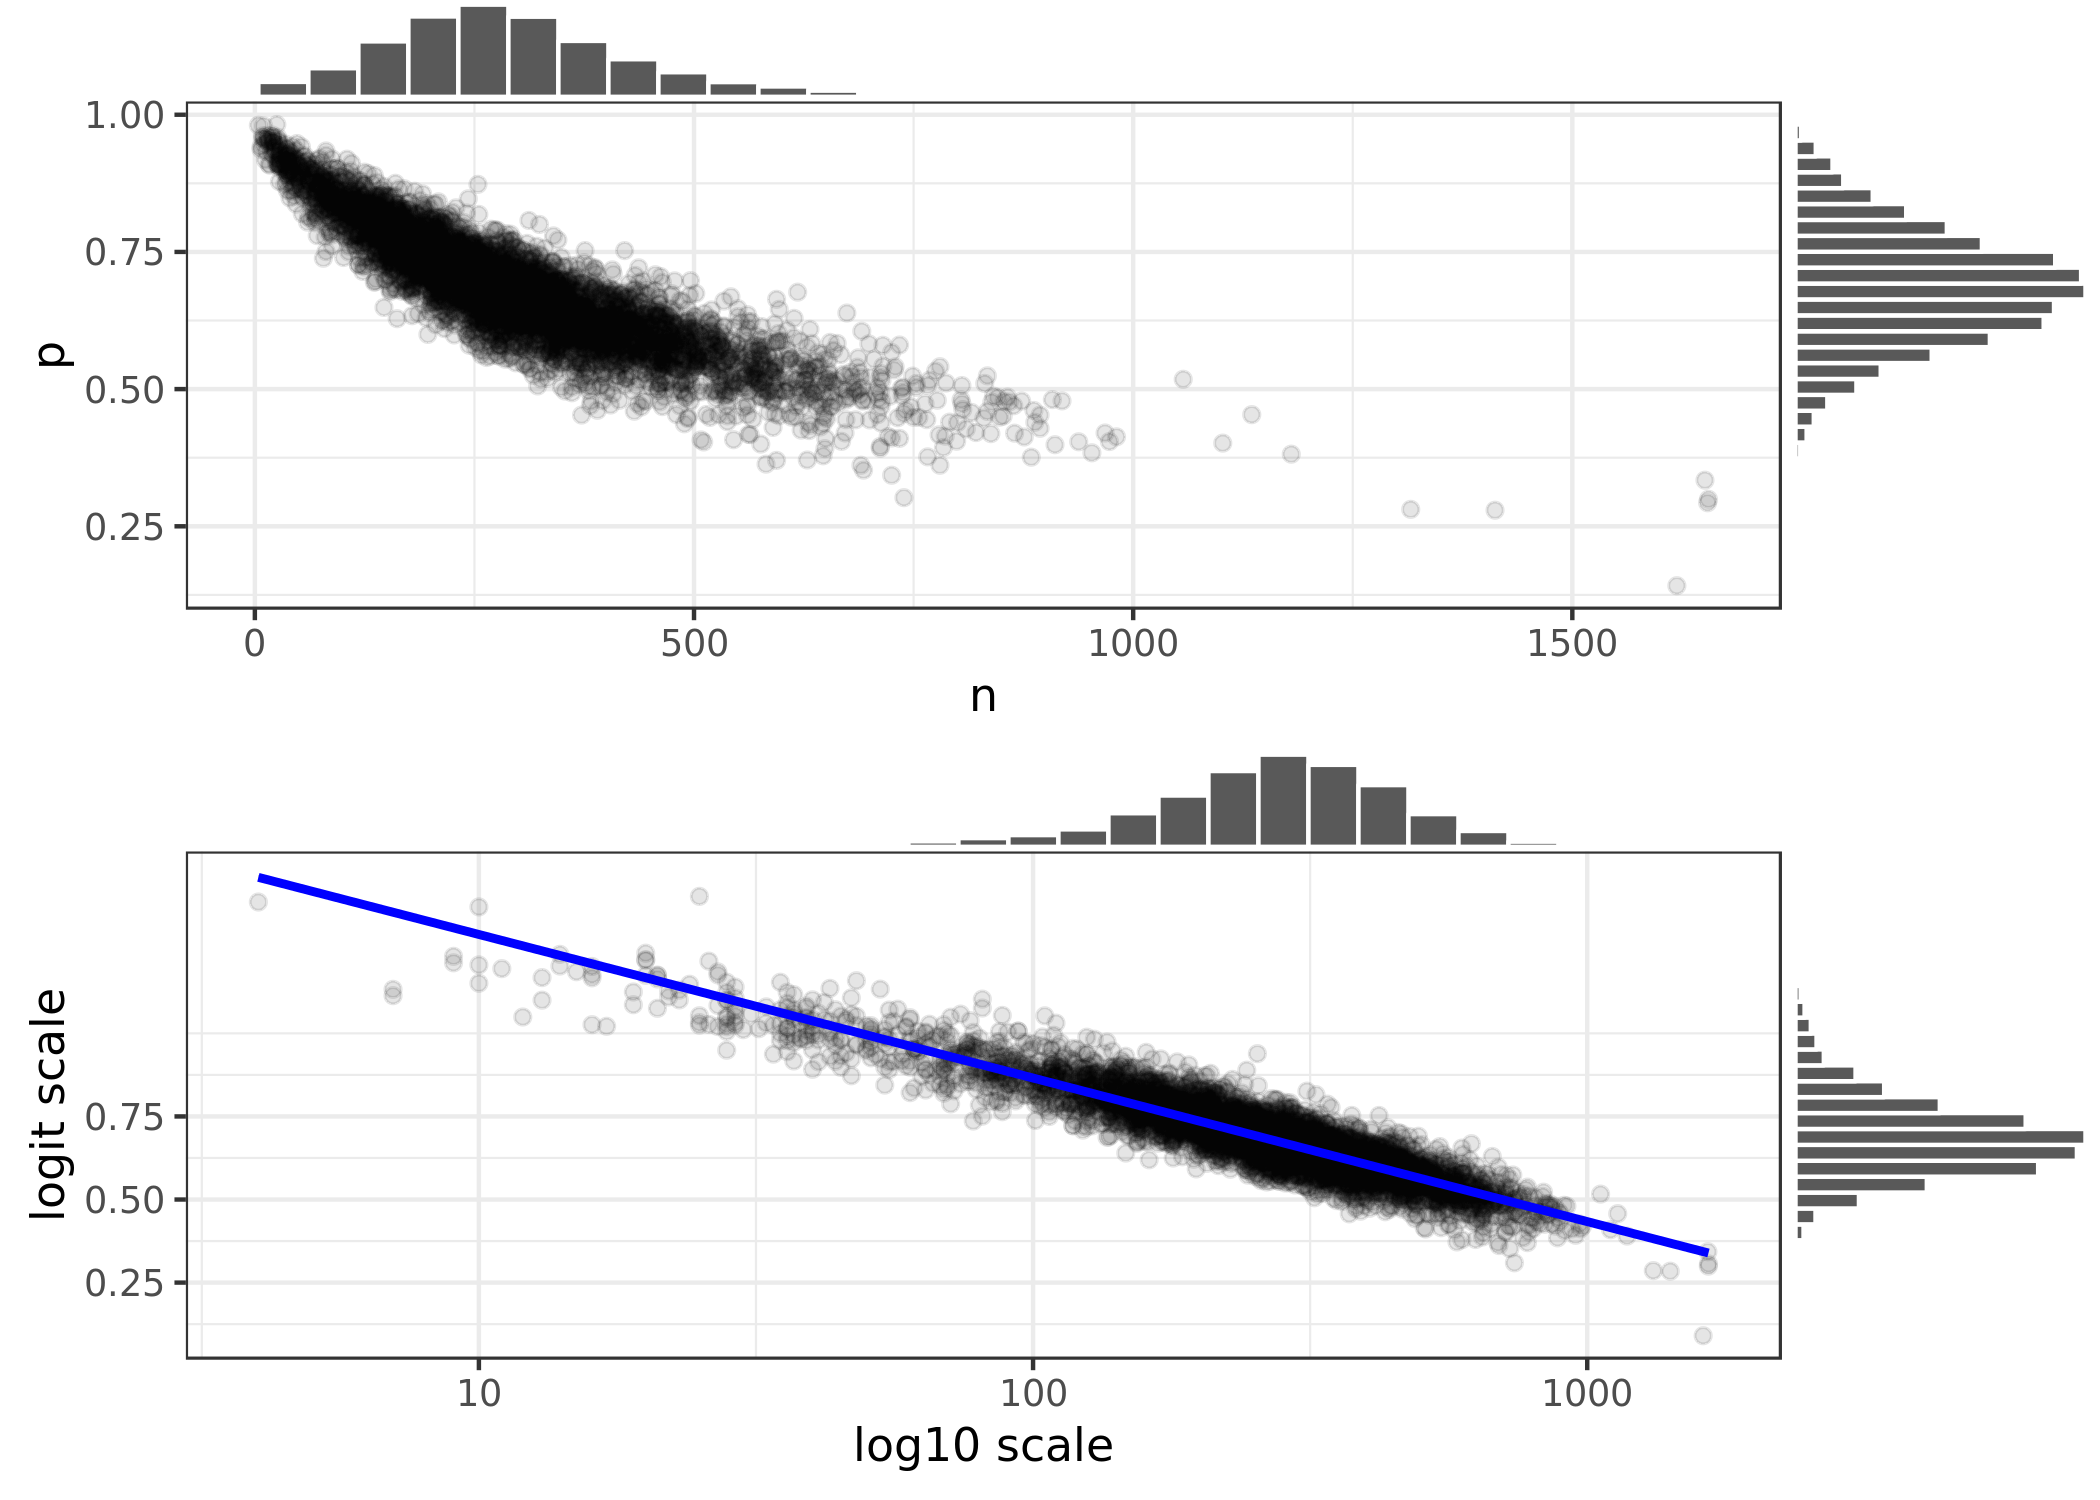
\includegraphics[width=0.9\linewidth]{ambrose_dissertation_files/figure-latex/ghostN-1} 

}

\caption{Ghost probabilities, the sum of document proportion of terms predicted to be present but are actually missing, by document length. Ghost probabilities are on log-odds scale, and document length is on $log_{10}$ scale. The blue line is a linear fit on transformed data.}\label{fig:ghostN}
\end{figure}

A document's ghost probability is related to the notion of residuals
that would help assess overall model goodness of fit. A document's per
term residual can be calculated as the observed minus the predicted
document term probability, a document's overall residual the sum of the
squares of the same. These residuals differ from the ghost probabilities
in that they also include the gap in prediction for the terms that do
appear in the original. Either can be used for diagnostic purposes. The
ghost probabilities draw attention to more absurd prediction errors,
while the residuals are more statistically precise. Table
\ref{tab:Kghost} shows the results of two separate linear regressions
which help to rank topics according to each of these goodness of fit
measures while controlling for the powerful effect of document length,
as well as the other topics. In each, the higher the ranking the more
documents within a topic are affected by poor fit. The results are not
consistent between the fit measures. For the ghost probabilities model,
the more a document is composed from topics 8, 2, 3, 5, and 1 the more
likely it is to be predicted to contain terms it does not actually
contain, while documents composed from topics 4, 9 and 6 are more likely
to have their terms accurately predicted. For the residuals model, only
topic 1 is expected to have a poorer fit, while drawing from topics 7,
4, 9, and 8 are all expected to improve document fit. The only topics
for which the direction of effect is in agreement between the models is
topic 1 contributing to bad fit, topics 4 and 9 contributing to good
fit, and topic 10 being neutral.

\begin{table}[!htbp] \centering 
  \caption{Logit of document by topic probability predicting A. logit of ghost probability or B. residual, controlling for log10 of document length} 
  \label{tab:Kghost} 
\begin{tabular}{@{\extracolsep{5pt}} lrrrr} 
\\[-1.8ex]\hline 
\hline \\[-1.8ex] 
Rank & A. Topic & Ghost p Coef. & B. Topic & Residual Coef. \\ 
\hline \\[-1.8ex] 
First & 8 &  0.0498 & 1 &  0.0142 \\ 
Second & 2 &  0.0391 & 10† & -0.0002 \\ 
Third & 3 &  0.0349 & 3† & -0.0018 \\ 
Fourth & 5 &  0.0216 & 6† & -0.0073 \\ 
Fifth & 1 &  0.0176 & 5† & -0.0087 \\ 
Sixth & 7† &  0.0054 & 2† & -0.0091 \\ 
Seventh & 10† & -0.0030 & 8 & -0.0141 \\ 
Eighth & 6 & -0.0177 & 9 & -0.0221 \\ 
Ninth & 9 & -0.0278 & 4 & -0.0245 \\ 
Tenth & 4 & -0.0324 & 7 & -0.0295 \\ 
\hline \\[-1.8ex] 
\multicolumn{5}{l}{† not significant at p < .001} \\ 
\multicolumn{5}{l}{Outcomes normalized to make ceofficents comparable.} \\ 
\end{tabular} 
\end{table}

\hypertarget{lower-tail-probability}{%
\subsection{Lower tail probability}\label{lower-tail-probability}}

A junk term is one that is common but unconcentrated or evenly
classified across all topics. This is the model's way of saying that it
belongs nowhere, which is to say everywhere. If such a term is truly
evenly distributed across topics and documents then the biases would
balance out. However we do not expect language to work this way; what is
more common is that junk terms are parts of suppressed topics, which
would emerge at a higher K, and that these topics are concentrated in
regions of the corpus. If this is true, they will bias upward fitted
topics that are correlated with the suppressed topic. If the suppressed
topic stood in a hierarchical relationship to one topic this would not
be a concern because in effect the child topic could be considered to be
partially constitutive of the parent topic at a lower resolution of K.
However in the expected case of more freely variable topics, unfitted
topics will bias upward the topics with which they are correlated.

Normally we expect a term that is taken up by one or a few topics to be
set to zero in the other topics. In order to prevent the estimation of
negative probability values, the quantity estimated is a transformation
of the probability that approaches but cannot meet or pass a zero limit.
In the STM model this transformation is the logarithm which is infinite
when transforming a probability of zero. When these estimates are
exponentiated to recover their associated probability, they will be
vanishingly small, and some may even be returned as zero due to machine
limits on the representation of small numbers. These psuedo zero
coefficients are no practical bother as they are not big enough to sum,
even in large numbers, to a significant probability. A psuedo zero
coefficient will be a large negative number on the logarithm scale,
whereas a junk coefficient, a small but nontrivial probability, will be
a smaller negative number.

Some back of the envelope calculations can illustrate the pitfalls of
junk terms. For argument's sake we can suppose a problematic junk
coefficient to be a function of the length of the global vocabulary
vector such that the bias it might introduce to a topic would appear in
a summation of some large portion of the global vector. Substantively, a
topic ought to be characterized by several dozen or perhaps a few
hundred terms, and because this is a feature of language and cognition
we would expect it to be invariant to the size of the global vocabulary.
However, as the global vocabularly grows the effect of junk terms as a
source of bias increases. In our case we retained 8,390 terms in the
global vocabularly vector. If conservatively we say that a topic is
described by as many as 500 terms, then the unused portion of the global
vector would be 1 - (500 / 8,390) or 94 percent of it.

Now we can consider how large a bias would need to be to be problematic.
A bias of five percent or a proportion of 0.05 could be more than enough
to for instance change a within-document topic ranking. What then is the
sum of the lower tail probabilities (LTP), less than the94th percentile,
of each of the topic by term vectors in our K = 10 model? Table
\ref{tab:k10tail} shows that the lower tail of the distribution ranges
from one quarter to one third of the total topic probability. These are
hardly insignificant portions of the classificatory power of the topics,
but in order for the junk vector to bias a particular document's topic
classification it would need to contain a large number of these terms,
the largest of these lower tail terms being on the order of four
hundreths of a percent. In the especially problematic case it would also
not contain terms in the head of the distribution.

\begin{table}[!htbp] \centering 
  \caption{Sum of topic by term probabilities below 94th percentile.} 
  \label{tab:k10tail} 
\begin{tabular}{@{\extracolsep{5pt}} lrr} 
\\[-1.8ex]\hline 
\hline \\[-1.8ex] 
k & LTP & Max. \\ 
\hline \\[-1.8ex] 
2 & 0.326 & 0.000436 \\ 
3 & 0.317 & 0.000492 \\ 
8 & 0.317 & 0.000434 \\ 
5 & 0.307 & 0.000421 \\ 
7 & 0.277 & 0.000381 \\ 
10 & 0.258 & 0.000383 \\ 
4 & 0.253 & 0.000390 \\ 
1 & 0.252 & 0.000436 \\ 
6 & 0.241 & 0.000398 \\ 
9 & 0.239 & 0.000400 \\ 
\hline \\[-1.8ex] 
\end{tabular} 
\end{table}

Table \ref{tab:worstdoc} illustrates the LTP problem for a document that
we expect to be poorly classified, that is, that has a large portion of
its explained words deriving from a topic's lower tail. The document in
question, a chapter from Mason and McCruden's ``Reading the Epistle to
the Hebrews'', is derived entirely from topic 2, which we may surmise is
about religion.\footnote{www.jstor.org/stable/10.2307/j.ctt1bhkpdr.8}
Here nearly a third of the terms explained by topic two come from the
lower tail. If we assume that these terms are representative of topics
other than religion, then we must conclude that the topic assignment of
this document is biased dramatically upward, that rather than being 100
percent about religion, it is in fact 66 percent about religion, and the
remainder is unexplained. In this case the corrected estimate does not
alter the topic ranking since there is no topic mixture to confuse.

\begin{table}[!htbp] \centering 
  \caption{Lower tail diagnostic for Mason and McCruden's "Reading the Epistle to the Hebrews"} 
  \label{tab:worstdoc} 
\begin{tabular}{@{\extracolsep{5pt}} lrrrrr} 
\\[-1.8ex]\hline 
\hline \\[-1.8ex] 
Topic & Topic Proportion & N Terms Explained & LTP & N from Lower Tail & N from Upper Tail \\ 
\hline \\[-1.8ex] 
2 & 0.999 & 298.597 & 0.325 & 97.130 & 201.466 \\ 
9 & 0.001 &   0.168 & 0.000 &  0.000 &   0.168 \\ 
1 & 0.000 &   0.058 & 0.000 &  0.000 &   0.058 \\ 
10 & 0.000 &   0.052 & 0.000 &  0.000 &   0.052 \\ 
7 & 0.000 &   0.047 & 0.000 &  0.000 &   0.047 \\ 
4 & 0.000 &   0.031 & 0.000 &  0.000 &   0.031 \\ 
8 & 0.000 &   0.023 & 0.000 &  0.000 &   0.023 \\ 
6 & 0.000 &   0.016 & 0.000 &  0.000 &   0.016 \\ 
3 & 0.000 &   0.008 & 0.000 &  0.000 &   0.008 \\ 
5 & 0.000 &   0.001 & 0.000 &  0.000 &   0.001 \\ 
\hline \\[-1.8ex] 
\end{tabular} 
\end{table}

If the terms in the lower tail are on the contrary about religion, then
the document may in fact be correctly classified. Figure
\ref{fig:worstterms} shows the lower tail terms from topic 2 that are
actually present in the text alongside those that are expected to be but
are note present. When sorted by the expected proportion, most of the
terms do not appear to be highly relevant to religion, though some--like
bishop, ritual, homilies, and hell--certainly are. When sorting by those
terms that are actually in the text--such as Levi, eschatological, and
messiah--the religious meaning is much more clear. These results suggest
that the 500 term threshhold may be too low for this topic, that it has
a very long list of relevant vocabulary. It is interesting to note that
the term ranking by original document frequency is more suggestive of
religious content, while the predicted frequency, of messiah for
instance, actually dilutes the term ranking. This is an indication of
imperfect fit, as a term like messiah was predicted to be less important
to the text than it actually is.

\begin{figure}

{\centering 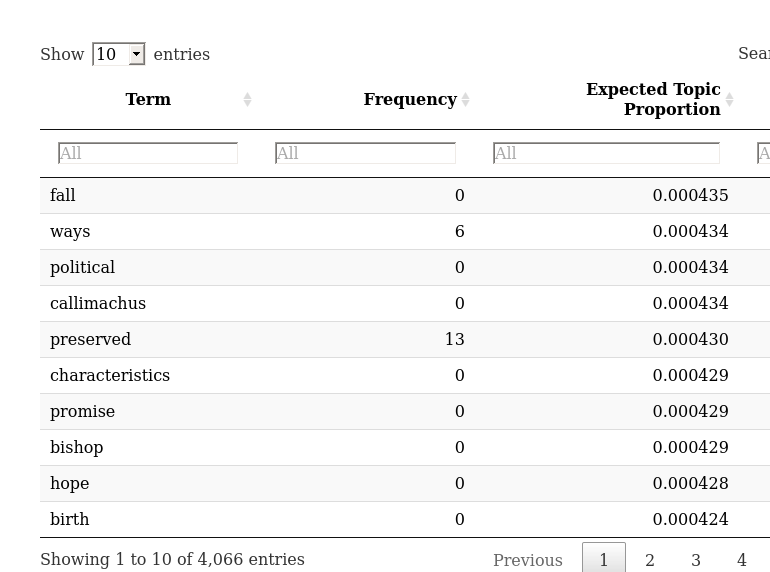
\includegraphics[width=0.9\linewidth]{ambrose_dissertation_files/figure-latex/worstterms-1} 

}

\caption{Terms from Mason and McCruden's "Reading the Epistle to the Hebrews" that are expected to derive from topic 2}\label{fig:worstterms}
\end{figure}

While we have already inspected the summary ranking of topics in terms
of a few measures of goodness of fit, it is helpful to observe the
within topic distributions of LTP, which will make the level of overlap
among topics more clear. First we will inspect the primary topic
classification, as it is common for researchers to reduce the document
by topic probability matrix to the primary classification. Then we will
look at each topic considering all LTPs at once, not just that of the
primary topic.

Figure \ref{fig:worstall} plots the distribution of a document's primary
topic classification, the topic with the highest document by topic
probability for each document, over the document LTP ranking. In other
words, every document is put in a line starting with the highest LTP and
ending with the lowest LTP. The documents are then labeled with their
main topic classification, and a histogram is drawn for each topic
according to counts in bins of 200 along this line. This design mimics
the satisficing behavior of the conventional reader during QVC. Topics
clustered toward the head (left) of the line are composed of poorly fit
documents, and those toward the tail (right) are composed of well fit
documents. The plot shows that some topics are cleanly separated, namely
topics 2, 5, 3, and 8 at the head from topics 9, 6, and 1 at the tail,
with topics 7, 10, and 4 in the middle.

\begin{figure}

{\centering 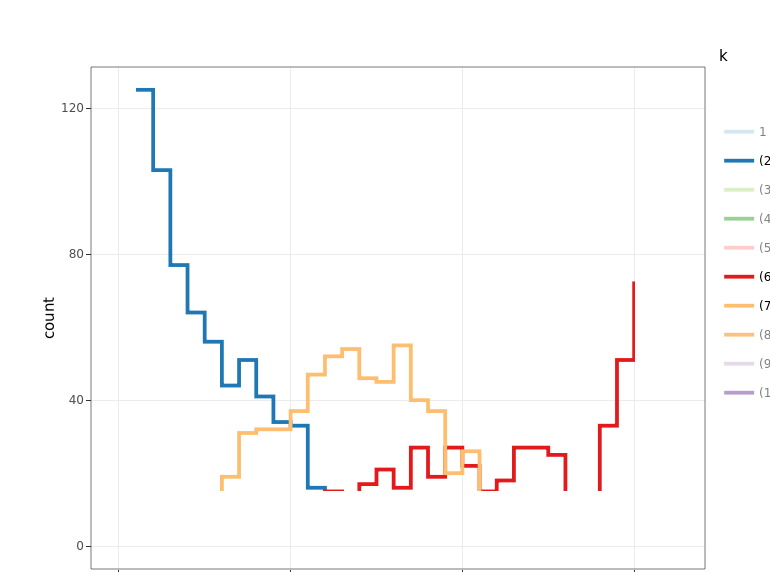
\includegraphics[width=0.9\linewidth]{ambrose_dissertation_files/figure-latex/worstall-1} 

}

\caption{Documents ranked by sum of lower tail probabilities by primary topic classification}\label{fig:worstall}
\end{figure}

For a different view of the problem taking all topic LTPs into account,
Figure \ref{fig:k10headtailp} shows the document distribution by topic
of the LTPs. Rather than looking at only the primary topic, here we
separate each document into its ten topic components, thus each document
is counted ten times, once for each of its topic LTPs. The logarithmic
scale helps us see a fairly even separation, at p = 0.00219, between the
portion of the corpus for which LTPs are and are not a serious
consideration. Below the sag between the two modes the LTPs are
vanishingly small and of no practical concern. Toward the upper mode,
however, we are concerned that the LTPs may be a source of
classification bias. This empirical separation visible on the log scale
is lower than the p = .05 standard that we considered above to be
practically problematic, which covers only the right hand tail of the
upper mode.

When looking at the LTP distribution for all document by topic pairs we
should expect an imbalance in favor of the upper mode, simply because
for every well classified document a few topics will be concentrated in
the head (low LTP) and the rest will be concentrated in the tail (high
LTP). Poorly classified documents will be drawn from the tails of most
topics. Here the lower mode accounts for 52 percent of document by topic
LTPs, so the distribution is more evenly split than we would expect with
strong document classification. This can be visually confirmed by the
nearly balanced shape of the black series, which shows the distribution
of all 10 * 6344 LTPs.

When comparing LTP distribution among individual topics there are clear
differences. Some topics have a much higher proportion of problematic
upper mode LTPs than others. For example, for topic 4 62 percent of
documents are poorly classified, while the same for topic 8 is 34.
Overall, topics 3, 8, and 6 have lower than average LTPs, topics 4, 9,
and 7 have higher than average LTPs, and topics 1 and 10 are close to
the average. Topics 2 and 5 stand out by being more dramatically split
between the two modes, with most of their documents having low LTPs but
a few having some of the highest in the sample.

\begin{figure}

{\centering 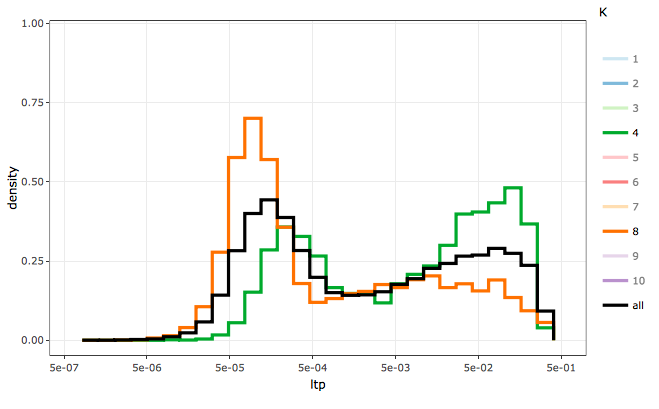
\includegraphics[width=0.9\linewidth]{img/k10headtail} 

}

\caption{Document distribution of sum of lower tail probabilities below 94th percentile by topic, $log_{10}$ scale}\label{fig:k10headtailp}
\end{figure}

Finally, the LTP distributions explored above are based on the arbitrary
cutoff at an index of 500, which we will recall was chosen to divide the
topic by term vectors into true and false segments. To show that topics
actually vary in the length of their relevant term lists, we can hold a
particular LTP proportion constant and see how many terms it takes to
reach that threshhold for each topic. Figure \ref{fig:elbow1p} shows the
cumulative proportion of the sorted term list for each topic up to an
LTP cutoff of one third, or an upper head probability of two thirds.
This cutoff is close to the maximum LTP at a constant index of 500, and
indeed we can confirm graphically what was said above that the topic
accounting for the maximum LTP is topic 2. Topics that reach the
threshold early tend to have a more concentrated term vector, that is,
have fewer terms accounting for the same amount of total probability.

Topic 6 reaches the threshhold first at an index of 315, which is a
considerably shorter list than 500. Topic 6 also starts with the highest
curve, meaning that it can be summarized by a short list of high
probability terms. Starting high does not necessarily mean a topic will
finish early, as evidenced by topic 10, which starts as high as topic 6
but grows more slowly and finishes late. The reverse is also possible,
as in the case of topic 10 that starts low and finishes early. Topics
can therefore cross each other in the explanatory power of their term
lists. Overall the topics are divided into a faster (topics 6, 9, 4, 10,
1, and 7) and a slower (topics 2, 3, 8, and 5) group.

\begin{figure}

{\centering 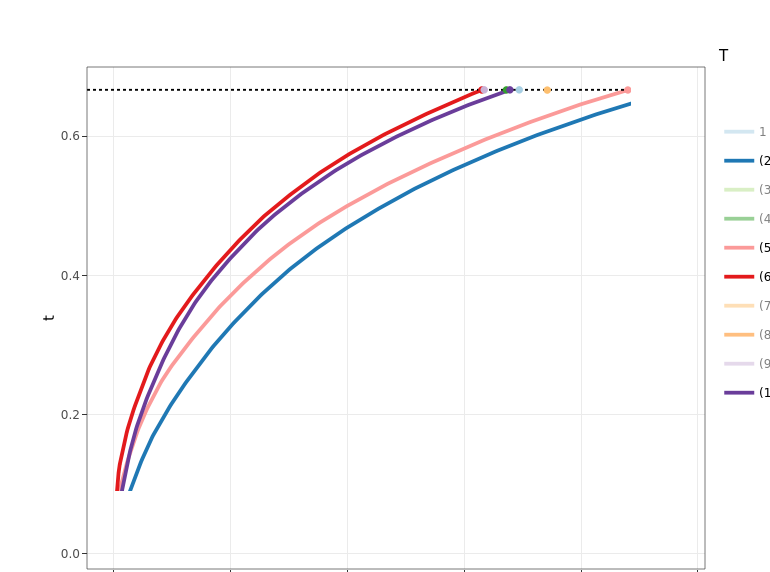
\includegraphics[width=0.9\linewidth]{ambrose_dissertation_files/figure-latex/elbow1p-1} 

}

\caption{Cumulative distribution of within topic term probabilities. Dotted line at p = 2/3}\label{fig:elbow1p}
\end{figure}

While there is no substantive reason to prefer topics with concentrated
term vectors, researchers tend to favor them because they are more
cognitively tractable. It is hard for analysts to make sense of hundreds
of terms; the more a topic can be adequately summarized by a short list
the more easily it is to reify. These diagnostic plots help to identify
the topics which may require additional attention to their lower ranked
terms.

\hypertarget{junk-threshhold}{%
\subsection{Junk threshhold}\label{junk-threshhold}}

Above we mentioned that probabilities in both the document by topic and
topic by term matrices are often expected to be zero but can not
actually be estimated as such due to the logarithmic transformation of
the original document by term data matrix. Zero predictions would make
the strict delineation between relevent and irrelevant terms or
documents easy even if it would still be an overly inclusive standard.
It would be helpful to find a natural breakpoint to establish when model
predictions are no longer relevant. It turns out that an empirical
threshold is obvious in the case of documents but not in the case of
terms. Figure \ref{fig:logit-theta} plots the progression of modal
separation of probabilities at growing levels of K. The modes are most
visible using the log-odds of the probability. When K is low the
distribution has three modes. This means

\begin{figure}

{\centering 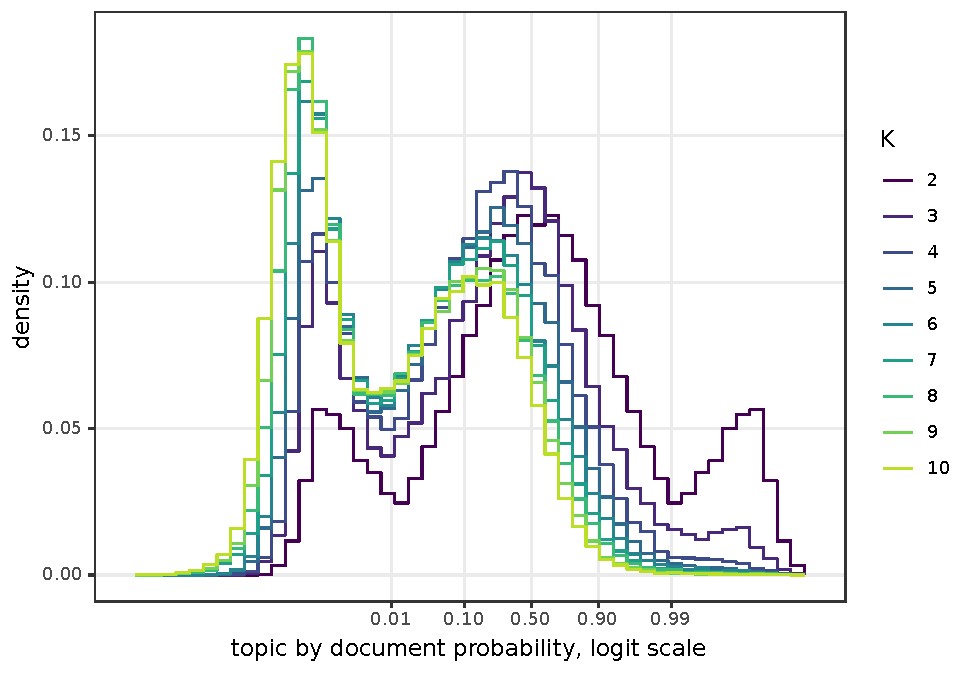
\includegraphics[width=0.9\linewidth]{ambrose_dissertation_files/figure-latex/logit-theta-1} 

}

\caption{As K increases so does separation among junk (lower mode), weak (central mode), and strong (upper mode) topic by document probabilities, logit scale}\label{fig:logit-theta}
\end{figure}

\begin{figure}

{\centering 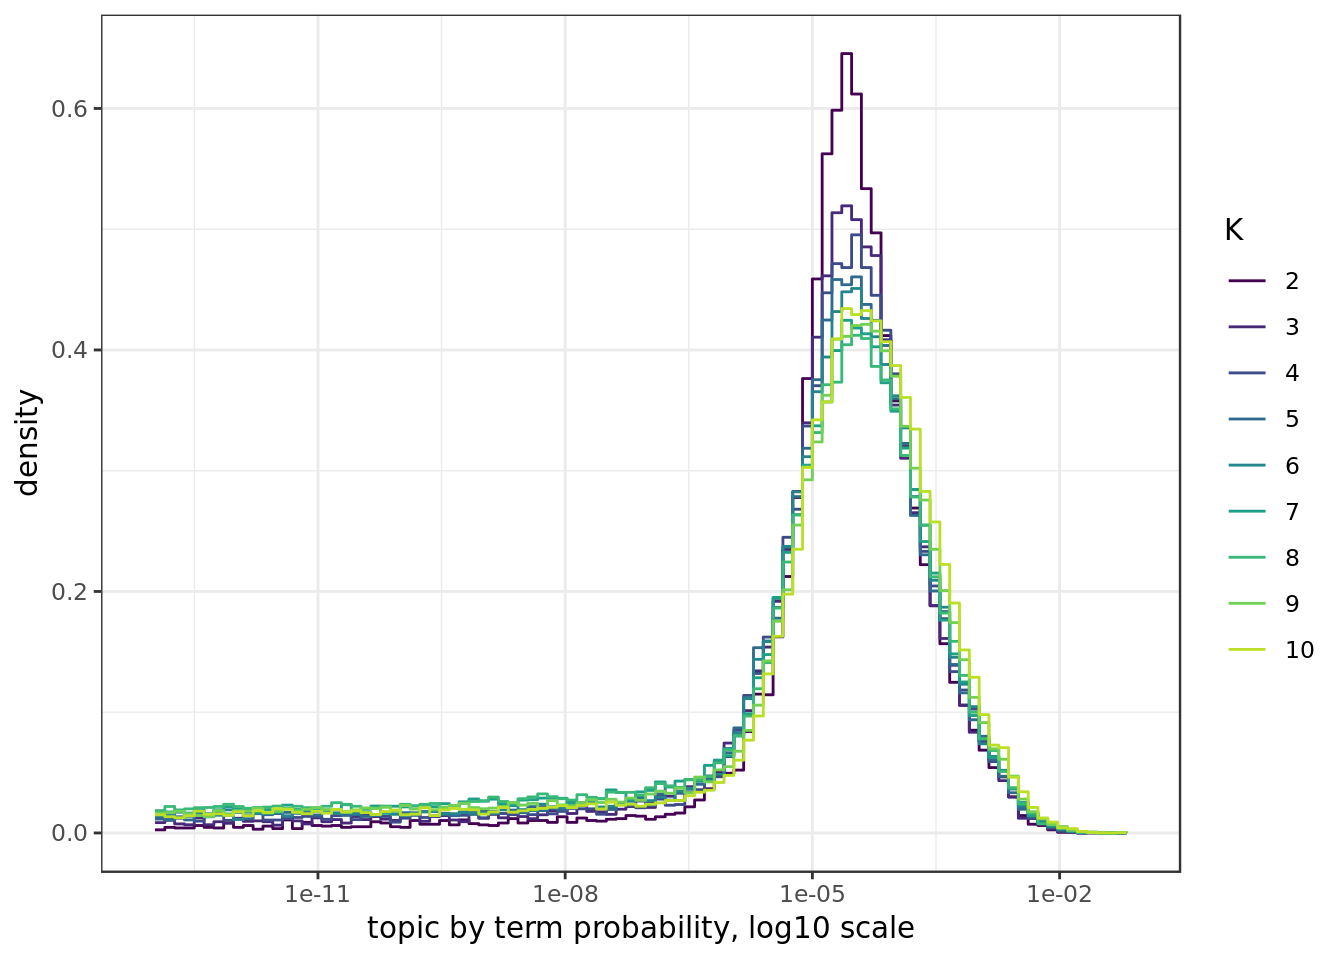
\includegraphics[width=0.9\linewidth]{ambrose_dissertation_files/figure-latex/log10-beta-1} 

}

\caption{As K increases, curve flattens toward more higher and more lower term probabilities, logit scale. Left tail truncated at logbeta > -30.}\label{fig:log10-beta}
\end{figure}

\hypertarget{concentration}{%
\subsection{Concentration}\label{concentration}}

While above it was possible to identify concentration during a
consideration of junk vectors, now we will measure concentration
directly..

\begin{figure}

{\centering 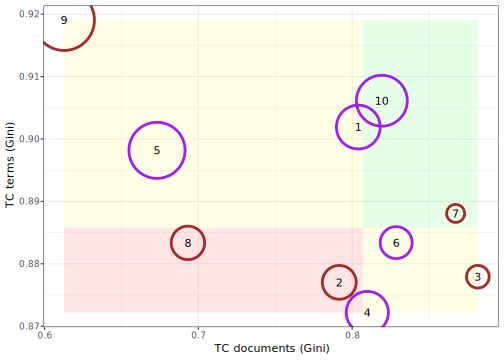
\includegraphics[width=0.9\linewidth]{ambrose_dissertation_files/figure-latex/top-gini-1} 

}

\caption{Topic concentrations (TC) within documents by TC within terms. Circles proportional to term frequency explained by each topic}\label{fig:top-gini}
\end{figure}

\begin{figure}

{\centering 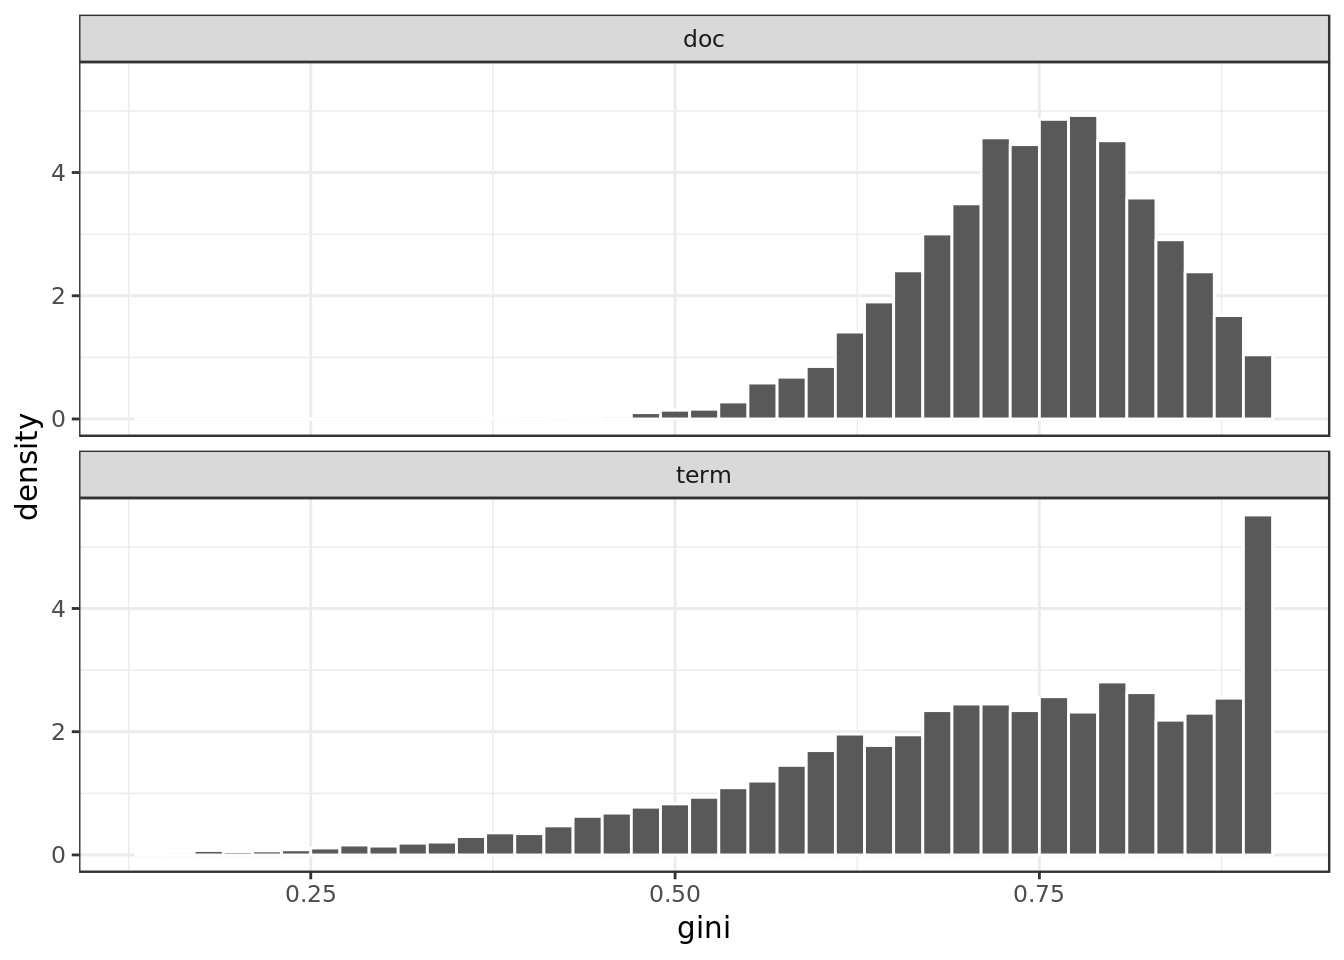
\includegraphics[width=0.9\linewidth]{ambrose_dissertation_files/figure-latex/doc-gini-1} 

}

\caption{Concentration of topic probabilities within A. documents and B. terms}\label{fig:doc-gini}
\end{figure}

\begin{figure}

{\centering 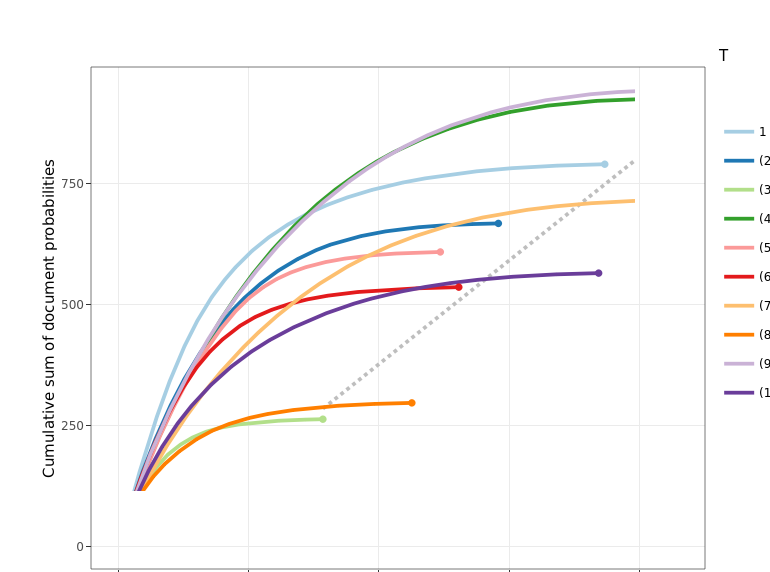
\includegraphics[width=0.9\linewidth]{ambrose_dissertation_files/figure-latex/elbow2-1} 

}

\caption{Cumulative distribution of within topic document probabilities.}\label{fig:elbow2}
\end{figure}

\hypertarget{topic-descent}{%
\subsection{Topic descent}\label{topic-descent}}

All topic models are mixture models in that they treat the observed
document by term frequencies as the outcome of multiple topics mixing
together in different proportions within documents. Whereas the flat
approach treats documents as mixtures, a hierarchical topic model treats
topics as mixtures as well. Here topics are mixtures of ancestor nodes
in a tree network of topics. A hierarchical model would, for instance,
obviate the procedure of removing common language syntax words such as
articles and prepositions because it could represent these as a root
node of all topics, indicating that all vocabularies appear in a partial
mixture of a language's basic syntax. A flat model retaining syntax
would burden the estimator with learning that syntax terms should be
distributed evenly across all topics. More substantively, a hierarchical
model applied to scholarship may help pick out fields that have various
empirical studies that are nonetheless united by common theory terms or
argumentative style words. Because substance in its detail can easily
swamp framing terminology by sheer frequency, flat topic model
estimators will tend to rends apart fields where novelty is a virtue and
classify them by their minutia rather than by their themes.

Models and software for hierarchical models have been developed
\citep{Teh2006Hierarchical, Roberts2015pkg}, but they are not yet in
common use by social scientists. Here we use a psuedo hierarchical model
in which we fit separate models at increasing levels of K, then we do
postestimation to measure the document level overlap among topics
between adjacent levels of K. We refer to this as topic decent, and it
shows how document classification evolves as K increases.

\begin{figure}

{\centering 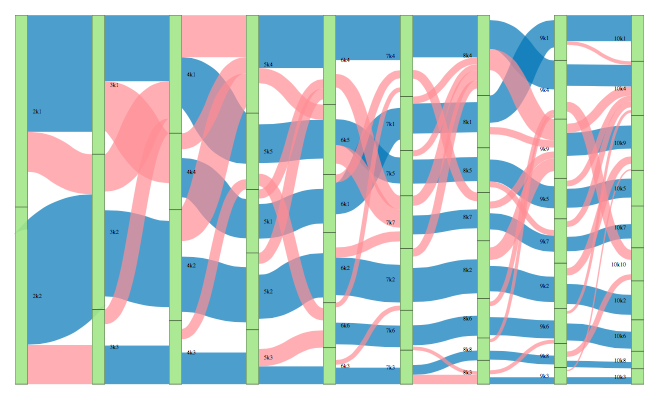
\includegraphics[width=1\linewidth]{img/genre-sankey} 

}

\caption{Sankey diagram of document overlap between topic models of increasing values of K.}\label{fig:sankey}
\end{figure}

\hypertarget{blind-qcv}{%
\subsection{Blind QCV}\label{blind-qcv}}

Contrary to the conventional approach of inspecting the topic by term
matrix first, I performed a blind QCV sorting test in which I tried to
recover the model classification without prior knowledge of topic
content. This test allows me to interpret topic content from whole texts
rather than from the decomposed topic by term matrix and gives an
opportunity to assess document classification quality prior to
developing a bias about what topic contents mean.

For each topic I created a list with 45 documents to supply five
comparison cases for each of the other nine topics. These lists were the
conventional document by topic rankings sorted in decreasing order of
topic probability. For each of the 45 unordered topic pairs I removed
five articles at random from the document list of each topic and
combined them to create a new randomly shuffled set of ten containing
documents from both topics. The validation task was simply to inspect
each document and attempt to recover the topic groupings, the logic
being that the better the document classification the easier the
sorting. Difficulty was measured by the chi squared probability of the
manual classifaction against the true classification. An additional
metric of difficulty, the amount of time required to complete the task,
was gathered as well but not used.

Each of the 45 sorting tasks was completed as quickly as possible, which
in practice meant skimming the first page of each document. If this was
enough to suggest the correct groupings the task would be finished. If
the status of some documents was unclear then a closer inspection of the
text would be necessary. Never was a document read closely, so topic
content is still what can be gleaned from a cursory skimming of the
text. Each document appeared only once within a particular topic's list
to avoid the bias of knowing how a document had already been classified
in a previous task. However, because a document could have appeared
twice or more if it was ranked in the top 45 documents of more than one
topic, some documents were seen twice. In these cases the bias would
serve to confuse rather than clarify since the classification would be
different between two instances of the same article.

\begin{figure}

{\centering 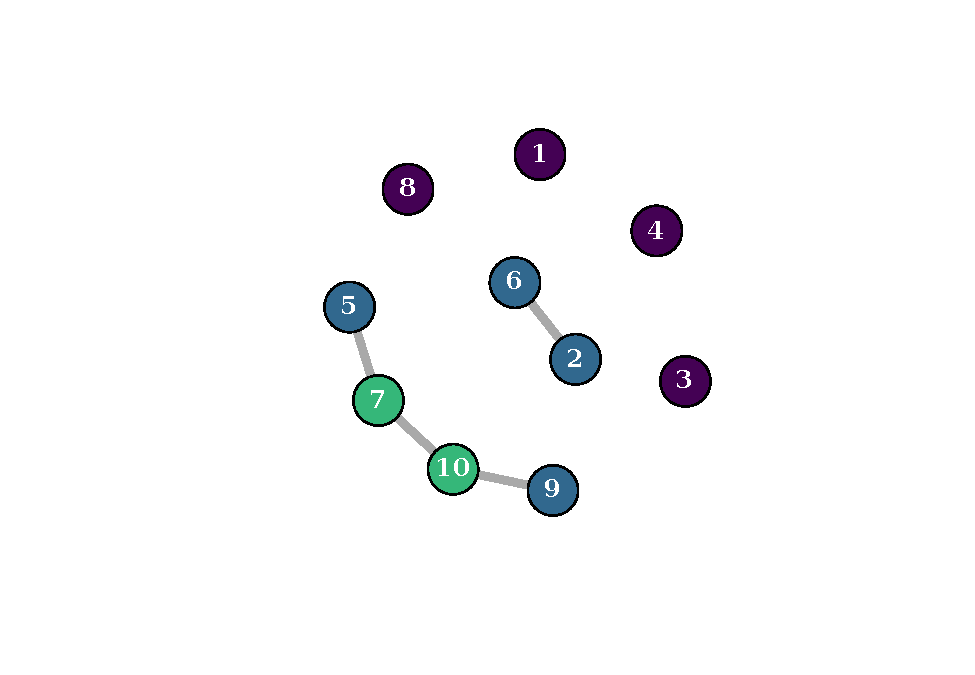
\includegraphics[width=0.9\linewidth]{ambrose_dissertation_files/figure-latex/man-con-1} 

}

\caption{Topic confusion network. Tied topics contained at least two errors in blind manual sorting test. Untied topics were perfectly separated. Colors represent a topic's number of imperfect tests.}\label{fig:man-con}
\end{figure}

Among the 45 different sorting tasks only two outcomes were observed. 41
tasks was performed perfectly (p = 0.0114), while in 4 tasks one error
was made, which is to say two documents were misclassified (p = 0.2059).
Figure \ref{fig:man-con} visualizes the pairwise outcomes as a confusion
network. Topics that are disconnected were sorted perfectly, while
topics that are connected were confused. The graph reveals some
variation in topic confusion, as two were confused twice, four were
confused once, and the remaining four were never confused.

It is not actually clear whether topic confusion is a function of
document misclassification or my lack of familiarity with topic content.
An added benefit of this procedure is that it began to establish a
theory of each topic by a direct inspection of bellwether texts, and
this growing familiarity decreases the task difficulty over the course
of the testing. In either event the results of this diagnostic provide a
basis for understanding interpretive difficulties later.

\hypertarget{reading-strata}{%
\section{Reading Strata}\label{reading-strata}}

\begin{verbatim}
.
   1    2    3    4 
2618 2409  703  614 
\end{verbatim}

\begin{center}\includegraphics[width=0.9\linewidth]{ambrose_dissertation_files/figure-latex/clusters-1} \end{center}

\begin{figure}

{\centering 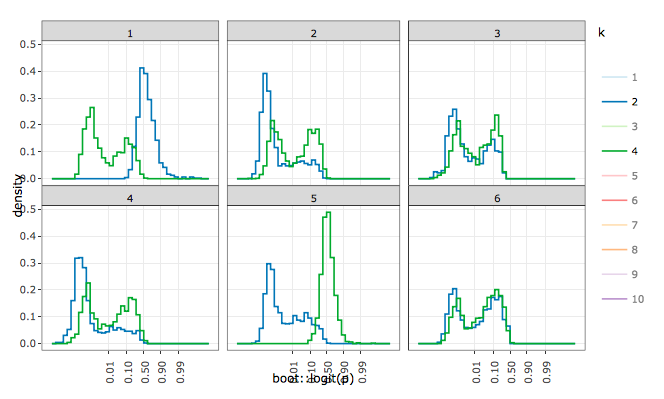
\includegraphics[width=0.9\linewidth]{img/clusters2} 

}

\caption{Topic by document probabilities within communities}\label{fig:clusters2}
\end{figure}

\hypertarget{results}{%
\section{Results}\label{results}}

\begin{table}[!htbp] \centering 
  \caption{Topic Rankings by Share of Corpus Explained} 
  \label{tab:topshare} 
\begin{tabular}{@{\extracolsep{5pt}} lr} 
\\[-1.8ex]\hline 
\hline \\[-1.8ex] 
Topic & Corpus Share \\ 
\hline \\[-1.8ex] 
9 & 0.1438 \\ 
4 & 0.1409 \\ 
1 & 0.1253 \\ 
7 & 0.119 \\ 
2 & 0.1057 \\ 
5 & 0.0973 \\ 
10 & 0.0871 \\ 
6 & 0.0848 \\ 
3 & 0.0495 \\ 
8 & 0.0465 \\ 
\hline \\[-1.8ex] 
\end{tabular} 
\end{table}

\begin{table}[!htbp] \centering 
  \caption{Most likely and most exclusive (anchorlike) terms} 
  \label{tab:prob-anc} 
\begin{tabular}{@{\extracolsep{5pt}} lrr} 
\\[-1.8ex]\hline 
\hline \\[-1.8ex] 
k & p & w \\ 
\hline \\[-1.8ex] 
1 & genre & bazerman, ablex, berkenkotter, classroom, curricular, curriculum \\ 
2 & god & aramaic, atque, auch, bakr, caliph, callimachus \\ 
3 & chinese & wang, bai, bao, beijing, bodhisattva, buddha \\ 
4 & fiction & aldiss, asimov, cyberpunk, darko, douglass, dystopia \\ 
5 & film & lms, blockbuster, bordwell, bros, cinema, cinematic \\ 
6 & music & accordion, balinese, chord, drummers, ethnomusicology, fiddle \\ 
7 & women & archie, aunque, femi, heteronormative, incestuous, lesbian \\ 
8 & les & cet, rien, toujours, ainsi, altro, aussi \\ 
9 & genre & hegel, kantian, menippean, schlegel, simplified, gadamer \\ 
10 & century & antwerp, booksellers, hogarth, netherlandish, pieter, rembrandt \\ 
\hline \\[-1.8ex] 
\end{tabular} 
\end{table}

\begin{verbatim}
Topic index maps to probability index like so:
      viz
 [1,]   9
 [2,]   4
 [3,]   1
 [4,]   7
 [5,]   2
 [6,]   5
 [7,]  10
 [8,]   6
 [9,]   3
[10,]   8
\end{verbatim}

\begin{figure}

{\centering \href{https://mercury.dlab.berkeley.edu:2018}{\includegraphics[width=1\linewidth]{ambrose_dissertation_files/figure-latex/genr-mod-viz-1} }

}

\caption{Topic Term Explorer, K=10}\label{fig:genr-mod-viz}
\end{figure}

\hypertarget{discussion}{%
\section{Discussion}\label{discussion}}

\bibliography{references.bib}


\end{document}
